\documentclass{sig-alternate-10pt-compact}

\usepackage{amsmath,amssymb}
\usepackage{url}
\usepackage{multirow}
\usepackage[usenames]{color}
\usepackage{algorithm}
\usepackage{algorithm}
\usepackage[noend]{algpseudocode}
\usepackage{times}
\usepackage{balance}
\usepackage{graphicx}
\usepackage{epstopdf}
\usepackage[tight,footnotesize]{subfigure}

\setlength{\pdfpagewidth}{8.5in}
\setlength{\pdfpageheight}{11in}


\DeclareMathOperator*{\argmax}{argmax}
\DeclareMathOperator*{\argmin}{argmin}

\newtheorem{cor}{Corollary}
\newtheorem{thm}{Theorem}
\newtheorem{definition}{Definition}
\newtheorem{lem}{Lemma}

\newcommand\fixme[1]{{\color{red} [#1]}}

\newcommand\hei{{h}}
\newcommand\dist{{L}}
\newcommand\beam{{\theta}}

\newcommand{\para}[1]{{\vspace{4pt} \bf \noindent #1 \hspace{2pt}}}
\newcommand\note[1]{{\color{red}#1}}
\newcommand\bedit[1]{#1}
\newcommand\htedit[1]{#1}
\newcommand\newed[1]{{\color{black}#1}}


\newenvironment{packed_itemize}{
\begin{list}{\labelitemi}{\leftmargin=1.3em}
  \setlength{\itemsep}{5pt}
  \setlength{\parskip}{0pt}
  \setlength{\parsep}{0pt}
  \setlength{\headsep}{0pt}
  \setlength{\topskip}{0pt}
  \setlength{\topmargin}{0pt}
  \setlength{\topsep}{0pt}
  \setlength{\partopsep}{0pt}  
}{\end{list}}

\begin{document}

\clubpenalty=10000 
\widowpenalty = 10000

\title{Control theoretic analysis of DCQCN and TIMELY}

\author{Paper \# XXX. Pages XX}

\maketitle
\begin{abstract}
Data center networks, and especially drop-free RoCEv2 networks require efficient
congestion control protocols. DCQCN (ECN-based) and TIMELY (delay-based) are two
recent proposals for this purpose.  In this paper, we analyze DCQCN and TIMELY
using fluid models and simulations, for stability and convergence. We uncover
several surprising behaviors of these protocols. For example, we show that DCQCN
exhibits non-monotonic stability behavior, and that TIMELY can converge to
stable regime with arbitrary unfairness. We propose simple fixes and parameter tuning
for stabilizing both protocols at the fair share point. Finally, using the
lessons learnt from the analysis, we address the broader question: are there
fundamental reasons to prefer either ECN or delay for end-to-end congestion
control in data center networks? We argue that ECN is a better congestion
signal, due to the way modern switches mark packets, and also due to a
fundamental limitation of end-to-end delay-based protocols.
\end{abstract}

\section{Introduction}

Large cloud service providers are turning to Remote DMA (RDMA) technology to
support their most demanding
applications~\cite{dcqcn,timely,tcp-bolt,erasure-storage,farm,pilaf}.  The
reason is that RDMA offers significantly higher bandwidth and lower latency than
the traditional TCP/IP stacks, while minimizing CPU
overhead~\cite{dcqcn,farm,timely}. 

In modern data centers, RDMA is deployed using the ROCEv2
standard~\cite{rocev2}. To ensure efficient operation, ROCEv2 eliminates packet
drops due to buffer overflow using Priority Flow Control (PFC)~\cite{pfc}.
Since there are no packet drops, any end-to-end congestion control protocol for
RoCEv2 networks must use either ECN markings, or delay as the congestion signal.
Last year, two protocols were proposed for this purpose, namely
DCQCN~\cite{dcqcn} and TIMELY~\cite{timely}. DCQCN uses ECN marking as a
congestion signal, while TIMELY measures changes to end-to-end delay.

% what we do.

In this paper, we analyze DCQCN and TIMELY for stability, convergence and
fairness. More importantly, using the insights drawn from the analysis, we
answer the broader question: are there fundamental reasons to prefer either ECN
or delay as the congestion signal in such environments?

% why we do it.

One of our motivations for analyzing these protocols is their potential for
widespread deployment, beyond large cloud providers.  DCQCN is implemented
entirely in Mellanox NICs, and drivers both Windows and Linux operating system
are available. Thus, anyone can deploy DCQCN in their data centers. While TIMELY
is not publically available, the core timing functionality it relies on is
supported by most modern NICs and their drivers.

Apart from this practical consideration, we are also driven by scientific
curiosity.  Numerous ECN and delay based congestion control protocols have been
proposed and analyzed before~\cite{ecn, tcp-vegas,
Hollot:PIController,misra2000fluid,hollot2001designing,misra:TAC2002,gorinsky2004feedback}.
However, barring a few recent exceptions~\cite{dctcp-analysis, qcn-analysis}
most prior work has been in the context of wide area networks.  Unfortunately,
neither ECN, nor delay based congestion control has seen widespread deployment
in the wide area Internet, for a variety of reasons. 

However, since RoCEv2 data center networks are drop-free, ECN or
delay-based congestion control is not just useful --- it is necessary. These
networks are a very different from the wide area Internet: the links have far
higher bandwidths, propagation delays are much lower, and the traffic is highly
bursty. Thus, protocols like DCQCN or TIMELY are likely to widespread deployment
in such networks.

We also note that while both DCQCN and TIMELY were developed for RoCEv2
networks, there is nothing RDMA-specific about either protocol, apart from the
fact that they both ignore the impact of packet drops. We believe that like
DCTCP~\cite{dctcp}, they are generally useful in any data center environment.

Thus, the time is ripe for analytical exploration of ECN and delay-based
congestion control protocols in this context; specifically to answer the
question we posed earlier.

% Methodology.

To this end, we analyze DCQCN and TIMELY using detailed fluid models and NS3
simulations. Our methodology is similar to the methodology used ny Alizadeh et.
al. for analyzing DCTCP~\cite{dctcp-analysis} and QCN~\cite{qcn-analysis}. Fluid
models are useful for analyzing properties such as stability, and for rapid
exploration of parameter space.  Simulations are useful for studying
packet-level dynamics and establishing the fidelity of the fluid model.  We will
publish our simulation code, as well the Matlab code used to solve the fluid
models.

% summary of contributions and findings.

We stress that it is not our goal to do a comparison of DCQCN and
TIMELY.  Such comparison makes little sense, since both protocols offer several
tuning knobs, and given a specific scenario, either protocol can be made to
perform as well as the other. Instead, we focus on understanding the basic
behavior of delay based and marking based protocols, understand the
tradeoffs and draw generic insights from the analysis.
Our key contributions, and findings are summarized as follows.

\para{DCQCN:} $(i)$ We extend the fluid model proposed in~\cite{dcqcn}, to
show that DCQCN has a unique fixed point, where flows converge to their fair
share. $(ii)$ We show that while DCQCN is generally stable around this
fixed point, as long as the feedback latency is low. The relationship between
stability and the number of competing flows is non-monotonic, which is very
different from TCP's behavior~\cite{misra:TAC2002}. DCQCN is stable for both
very small, and very large number of flows, and tends to be unstable in between;
especially if the feedback latency is high.  $(iii)$ Using a discrete model, we
who that for typical parameter values, DCQCN converges to the aforementioned
fixed point within 100ms.

\para{TIMELY:} $(i)$ We develop a fluid model for TIMELY, and validate it using
simulations. $(ii)$ The fluid model reveals that since TIMELY relies on {\em RTT
gradient} as congestion signal, it can have infinite fixed points, resulting in
arbitrary unfairness.  $(iii)$ We propose a simple fix to remedy this problem,
and show that the modified version of TIMELY is stable, and converges to a fixed
point within \fixme{xxx}. 

\para{General results:} $(i)$ We show that for both variants of
the protocols studied, the fixed point of the queue length (and hence
feedback delay) increases with the number of flows $(ii)$ Higher
delays are undesirable both from an application perspective as well as
difficulty in controlling the loop. To fix that, we show that using
integral control, e.g. the PI~\cite{Hollot:PIController}-like
marking scheme, we can make 
the queue length (and hence delay) independent of the number of contending
flows. $(iii)$ In controlling the queue length to a fixed point, we
derive a \emph{fundamental} result for congestion control: for a
distributed protocol that uses only delay as the feedback signal, you
can achieve either fairness or a guaranteed delay, but not both simultaneously. For a
protocol that employs ECN marking based network feedback, you can
achieve both. $(iv)$ We discuss the pros and cons of the use of hardware rate limiters
(DCQCN uses them, TIMELY does not).


\section{Background}
The Remote Direct Memory Access (RDMA) technology offers high throughput(40Gbps
or more), low latency (few $\mu$s), and low CPU overhead (1-2\%), by bypassing
the end-host kernels during data transfer. Instead, network interface cards
(NICs) transfer data in and out of pre-registered memory buffers at the two end
hosts. The networking protocol is implemented entirely on the NICs.

Modern data center networks deploy RDMA using the RDMA over Converged Ethernet
V2 (RoCEv2)~\cite{rocev2} standard.  RoCEv2 requires a lossless (or, more
accurately, drop-free) L2 layer. Ethernet can be made drop-free using Priority
Flow Control (PFC)~\cite{pfc}. PFC prevents buffer overflow on Ethernet switches
and NICs. The switches and NICs track ingress queues. When the queue exceeds a
certain threshold, a PAUSE message is sent to the upstream entity. The uplink
entity then stops sending on that link till it gets an RESUME message.  PFC is a
blunt mechanism, since it does not operate on a per-flow basis. This leads to
several well known problems such as head-of-the-line
blocking~\cite{dcqcn,tcp-bolt}. 

PFC's problems can be mitigated using per-flow congestion control. Since PFC
eliminates packet drops due to buffer overflow, either ECN or increase in RTT
are the only two available ``end-to-end'' congestion signals.  DCQCN relies on
ECN, while TIMELY relies on RTT changes.

As noted earlier, neither DCQCN, nor TIMELY are RDMA-specific. Thus the analysis
in the rest of the paper makes no reference to RoCEV2 or RDMA.


\section{DCQCN}

\subsection{Model}

\begin{equation}
\small
p(t) = \left\{ \begin{array}{ll}
{\rm{0,}} & q(t) \le {K_{\min }}\\
\frac{{q(t) - {K_{\min }}}}{{{K_{\max }} - {K_{\min }}}}{p_{\max }}, & {K_{\min }} < q(t) \le {K_{\max }}\\
{\rm{1,}} & q(t) > {K_{\max }}
\end{array} \right.
\label{eq:mark}
\end{equation}
\begin{equation}
\small
\frac{{dq}}{{dt}} = N{R_C}(t) - C
\label{eq:q}
\end{equation}
\begin{equation}
\small
\frac{{d\alpha }}{{dt}} = \frac{g}{{\tau '}}\left( {\left( {1 - {{(1 - p(t - \tau *))}^{\tau '{R_C}(t - \tau *)}}} \right) - \alpha (t)} \right)
\label{eq:alpha}
\end{equation}
\begin{equation}
\small
\begin{split}
\frac{{d{R_T}}}{{dt}} = & - \frac{{{R_T}(t) - {R_C}(t)}}{\tau }\left( {1 - {{(1 - p(t - \tau *))}^{\tau {R_C}(t - \tau *)}}} \right) \\
& + {R_{AI}}{R_C}(t - \tau *)\frac{{{{(1 - p(t - \tau *))}^{FB}}p(t - \tau *)}}{{{{(1 - p(t - \tau *))}^{ - B}} - 1}} \\
& + {R_{AI}}{R_C}(t - \tau *)\frac{{{{(1 - p(t - \tau *))}^{FT{R_C}(t - \tau *)}}p(t - \tau *)}}{{{{(1 - p(t - \tau *))}^{ - T{R_C}(t - \tau *)}} - 1}}
\end{split}
\label{eq:target}
\end{equation}
\begin{equation}
\small
\begin{split}
\frac{{d{R_C}}}{{dt}} = & - \frac{{{R_C}(t)\alpha (t)}}{{2\tau }}\left( {1 - {{(1 - p(t - \tau *))}^{\tau {R_C}(t - \tau *)}}} \right) \\
 & + \frac{{{R_T}(t) - {R_C}(t)}}{2}\frac{{{R_C}(t - \tau *)p(t - \tau *)}}{{{{(1 - p(t - \tau *))}^{ - B}} - 1}} \\ 
 & + \frac{{{R_T}(t) - {R_C}(t)}}{2}\frac{{{R_C}(t - \tau *)p(t - \tau *)}}{{{{(1 - p(t - \tau *))}^{ - T{R_C}(t - \tau *)}} - 1}}
\end{split}
\label{eq:current}
\end{equation}

\subsection{Model validation}

\subsection{Stability analysis}

\para{Fixed point.} We denote:

\begin{equation}
\begin{array}{l}
a(t) = 1 - {(1 - p(t))^{\tau {R_C}(t)}},b(t) = \frac{{p(t)}}{{{{(1 - p(t))}^{ - B}} - 1}},\\
c(t) = \frac{{{{(1 - p(t))}^{FB}}p(t)}}{{{{(1 - p(t))}^{ - B}} - 1}},d(t) = \frac{{p(t)}}{{{{(1 - p(t))}^{ - T{R_C}(t)}} - 1}},\\
e(t) = \frac{{{{(1 - p(t))}^{FT{R_C}(t)}}p(t)}}{{{{(1 - p(t))}^{ - T{R_C}(t)}} - 1}}
\end{array}
\end{equation}

DCQCN has a unique fixed point:

\begin{equation}
\small
{R_C^*} = \frac{C}{N}
\end{equation}
\begin{equation}
\small
\alpha^*  = 1 - {(1 - p)^{\frac{{\tau 'C}}{N}}}
\end{equation}
\begin{equation}
\small
{R_T^*} = \frac{C}{N} + \frac{{a\alpha }}{{(b + d)\tau }}
\end{equation}

\begin{equation}
\small
{q^*} = \frac{{{p^*}}}{{{p_{max}}}}\left( {{K_{max}} - {K_{min}}} \right) + {K_{min}}
\end{equation}

$p^*$ is determined by:
\begin{equation}
\small
\frac{{{a^2}\alpha }}{{(b + d)(c + e)}} = \frac{{{\tau ^2}{R_{AI}}C}}{N}
\end{equation}

We obtain the taylor series around $p=0$ of the left hand side:
\begin{equation}
\small
\frac{{{a^2}\alpha }}{{(b + d)(c + e)}} = \frac{{{C^3}{\tau ^2}\tau '}}{{{N^3}{{\left( {\frac{1}{B} + \frac{N}{{CT}}} \right)}^2}}}{p^3} + O\left( {{p^4}} \right)
\end{equation}

\begin{equation}
\small
{p^*} = \sqrt[3]{{\frac{{{R_{AI}}{N^2}}}{{\tau '{C^2}}}{{\left( {\frac{1}{B} + \frac{N}{{CT}}} \right)}^2}}}
\end{equation}

\para{Stability analysis.} 
We linearize the system by $\delta {R_C}(t) = {R_C}(t) - R_C^*$, $\delta {R_C}(t) = {R_C}(t) - R_C^*$,
$\delta p(t) = p(t) - p^*$, $\delta \alpha (t) = \alpha (t) - \alpha^*$, and $A = \left( {\frac{1}{B} + \frac{1}{{TR_C^*}}} \right)$.

\begin{equation}
\small
\begin{array}{l}
s{R_C}(s) - \delta {R_C}(0) = \left( { - \frac{1}{2}{{(R_C^*)}^2}{\alpha ^*} - \left( {\frac{1}{2} + \frac{A}{4}} \right)R_C^*R_T^* + \left( {\frac{1}{2} + \frac{A}{4}} \right){{(R_C^*)}^2}} \right){e^{ - s\tau *}}p(s)\\
 + \left( { - \frac{1}{2}{p^*}R_C^*{\alpha ^*} - \frac{A}{2}R_C^* + \left( {\frac{1}{2} + \frac{A}{4}} \right){p^*}R_C^*} \right){e^{ - s\tau *}}{R_C}(s)\\
 + \left( { - \frac{1}{2}{p^*}R_C^*{\alpha ^*} - \frac{A}{2}R_C^* + \frac{A}{2}R_T^* + \left( {\frac{1}{2} + \frac{A}{4}} \right){p^*}R_C^* - \left( {\frac{1}{2} + \frac{A}{4}} \right){p^*}R_T^*} \right){R_C}(s)\\
 - \frac{1}{2}{p^*}{(R_C^*)^2}\alpha (s)\\
 + \left( {\frac{A}{2}R_C^* - \left( {\frac{1}{2} + \frac{A}{4}} \right){p^*}R_C^*} \right){R_T}(s)
\end{array}
\end{equation}


\subsection{Convergence analysis}

\subsection{Discussion}


\vspace{-0.5em}
\section{TIMELY}

TIMELY~\cite{timely} is an end-to-end, rate-based congestion control algorithm
that uses changes in RTT as a congestion signal.  It relies on NIC hardware to
ontain fine-grained RTT measurements. RTT is estimated once per completion
event~\cite{rocev2}, which signals the successful transmission of a chunk
(16-64KB) of packets. Upon receiving a new RTT sample, TIMELY computes new rate
for the flow, as shown in Algorithm \ref{fig:timely_algo}.  If the new RTT
sample is less than ($T_{low}$), TIMELY increases send rate additively by
$\delta$. If the new sample is more than ($T_{high}$), rate is decreased
multiplicatively by $\beta$. If the new sample is between $T_{low}$ and
$T_{high}$, the rate change depends on the RTT gradient. The gradient is defined
as the normalized change between two successive RTT samples. If the gradident is
positive (i.e. RTT is increasing), sending rate is reduced multiplicatively by
$\beta \times normalized_gradient$.  Otherwise, it is increased additively by
$\delta$.

TIMELY implemeantion does not use hardware rate limiters. Rate control is done
by spacing chunks of data. Flows do not start at line rate. If there are N
active flows at a sender, a new flow starts at rate C/(N+1), where C is the
interface link bandwidth~\cite{timely:private}.

\begin{algorithm}[t]
\footnotesize
{
\begin{algorithmic}[1]
%\Procedure{CalcRate}{$newRTT$}
\State $newRTTDiff \gets newRTT - prevRTT$
\State $prevRTT \gets newRTT$
\State $rttDiff \gets (1-\alpha) \cdot rttDiff + \alpha \cdot newRTTDiff$
\State $rttGradient = rttDiff/D_{minRTT}$
\If {$newRTT < T_{low}$}
        \State $rate \gets rate + \delta$
\ElsIf {$newRTT > T_{high}$}
        \State $rate \gets rate \cdot  (1 - \beta \cdot (1 - T_{high}/newRTT))$
\ElsIf {$rttGradiant \le 0$}
        \State $rate \gets rate + \delta$
\Else
        \State $rate \gets rate \cdot (1 - \beta \cdot rttGradient)$
\EndIf 
%\EndProcedure
\end{algorithmic}
}
\caption{TIMELY rate calculation}
\label{fig:timely_algo}
\end{algorithm}


\subsection{Model}

We have developed a fluid model of TIMELY. It is shown in
Tables~\ref{tab:timely_var} and \ref{tab:timely_param} and
Figure~\ref{fig:timely_model}.  The model considers N flows, traversing a single
bottleneck link. The model assumes that TIMELY is triggered
before\footnote{Unlike~\cite{dcqcn}, ~\cite{timely} does not specify how to set
buffers to ensure this, but we assume that it can be done.} PFC, and hence
ignores the impact of PFC.

Equation~\ref{eq:timely_q} describes the queue behavior.
Equation~\ref{eq:timely_r} describes rate computation. For simplicity, we ignore
the hyperactive increase phase. When RTT is between$T_{low}$ and $T_{high}$, the
rate computation depend on RTT gradient, which evolves according to
Equation~\ref{eq:timely_g}.  The equation captures the EWMA filter, as well as
normalization. Since the gradient is the difference between the current and the
previous RTT sample, it depends on two queue lengths in past: one at time $t -
\tau'$, and one at time $t - \tau'-\tau\*$. The value of $\tau'$ and $\tau*$
depend on past transmission rates, but to simplify the model, we approximate
their calculation as shown in Equations~\ref{eq:timely_taus} and
\ref{eq:timely_taup}.  Equation~\ref{eq:timely_taus} captures the fact that the
TIMELY implementation updates rate at most once per $D_{minRTT}$.

\begin{table}[t]
\center
{
\footnotesize
{
\begin{tabular}{|c|c|} \hline
Variable & Description \\ \hline
$R$ & Rate \\ \hline
$g$ & RTT gradient\\ \hline
$q$ & Queue Size \\ \hline
$t$ & Time \\ \hline
$\tau*$ & Rate update interval \\ \hline
$\tau'$ & Feedback delay \\ \hline
\end{tabular}
}
}
\caption{TIMELY Fluid model variables}
\label{tab:timely_var}
\end{table}

\begin{table}[t]
\center
{
\footnotesize
{
\begin{tabular}{|c|c|} \hline
Parameter & Description \\ \hline
$N$ & Number of flows at bottleneck\\ \hline
$C$ & Bandwidth of bottleneck link\\ \hline
$\alpha$ & EWMA smoothing factor\\ \hline
$\delta$ & Additive increase step\\ \hline
$\beta$ & Multiplicative decrease factor\\ \hline
$T_{low}$ & Low threshold\\ \hline
$T_{high}$ & High threshold\\ \hline
$D_{minRTT}$ & Minimum RTT for normalization \\ \hline
$D_{prop}$ & Propagation delay \\ \hline
\end{tabular}
}
}
\caption{TIMELY Fluid model parameters}
\label{tab:timely_param}
\end{table}

\begin{figure}[h]
\fbox
{
\begin{minipage}{\columnwidth}
\begin{equation}
\small
\frac{{dq}}{{dt}} = \sum_{i} R(t) - C\\
\label{eq:timely_q}
\end{equation}
\begin{equation}
\small
\frac{{dR_i}}{{dt}} = \left\{ \begin{array}{ll}
\frac{\delta }{{\tau *}}, & q(t - \tau ') < C*{T_{low}}\\
\frac{\delta }{{\tau *}}, & g \le 0\\
 - \frac{{g\beta }}{{\tau *}}R_i(t), & g > 0\\
 - \frac{\beta }{{\tau *}}(1 - \frac{{C*{T_{high}}}}{{q(t - \tau ')}})R_i(t), & q(t - \tau ') > C*{T_{high}}
\end{array} \right.\\
\label{eq:timely_r}
\end{equation}
\begin{equation}
\small
\frac{{dg}}{{dt}} = \frac{\alpha }{{\tau *}}( - g(t) + \frac{{q(t - \tau ') - q(t - \tau ' - \tau *)}}{{C*{D_{\min RTT}}}})\\
\label{eq:timely_g}
\end{equation}
\begin{equation}
\small
\tau * = \max \{ \frac{{Seg}}{R},{D_{\min RTT}}\} \\
\label{eq:timely_taus}
\end{equation}
\begin{equation}
\small
\tau ' = \frac{q}{C} + \frac{{Seg}}{R} + {D_{prop}}
\label{eq:timely_taup}
\end{equation}
\end{minipage}
}
\caption{TIMELY fluid model}
\label{fig:timely_model}
\end{figure}

\para{Model Validation:}
Since we do not have access to TIMELY implemenation,
Figure~\ref{fig:timely_model_validation} compares the TIMELY fluid model with
the packet-level simulations using the NS3 simulator~\cite{ns3}. The parameters
values are shown in Table~\ref{tab:timely_model_validation}, and are based on
guidance provided in\cite{timely}.  We model a simple topology, in which N
senders, connected to a switch, send to a single receiver, also connected to
that switch. The starting rate for each flow is set to be 1/N of the link
bandwidth. 

We see the fluid model and the simulator are in good agreement, apart from some
time shift in queue behavior. The queue peaks at roughly 70KB, which corresponds
to 56$\mu$s at 10Gbps. As one would expect, this is close to the $T_{min}$.

\begin{table}[t]
\small
\center
\begin{tabular}{c|c}
Parameter & Value \\ \hline
C & 10Gbps \\ 
$T_{low}$ & 50 $\mu$s \\ 
$T_{high}$ & 500 $\mu$s \\
$D_{minRTT}$ & 20 $\mu$s \\
$\beta$ & 0.8 \\
$\alpha$ & 0.875 \\
$\delta$ & 10Mbps
\end{tabular}
\caption{TIMELY parameter values for model validation}
\label{tab:timely_model_validation}
\end{table}

\begin{figure}[t]
\center
\subfigure[N=2] { 
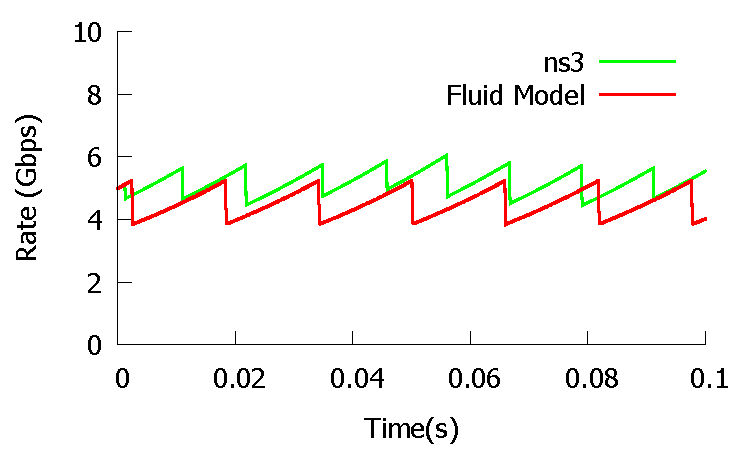
\includegraphics[width=0.45\columnwidth]{figures/timely_validation_2_rate.pdf}
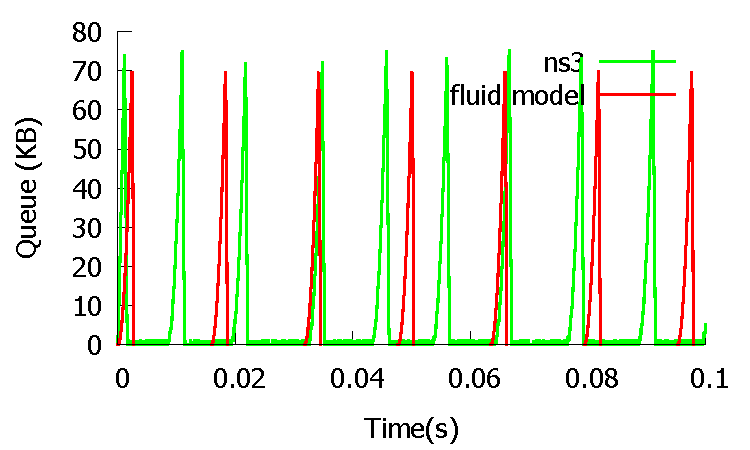
\includegraphics[width=0.45\columnwidth]{figures/timely_validation_2_q.pdf}
}
\subfigure[N=10] { 
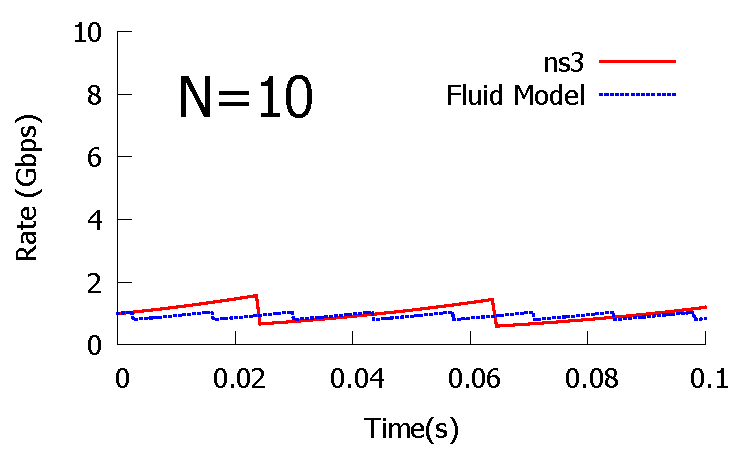
\includegraphics[width=0.45\columnwidth]{figures/timely_validation_10_rate.pdf}
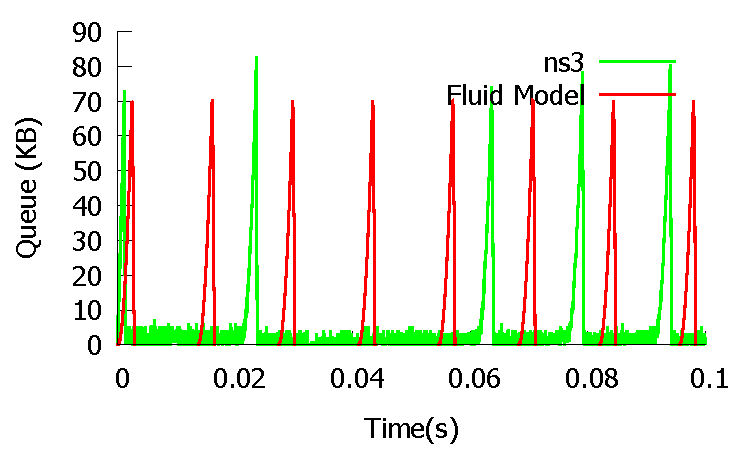
\includegraphics[width=0.45\columnwidth]{figures/timely_validation_10_q.pdf}
}
\subfigure[N=20] { 
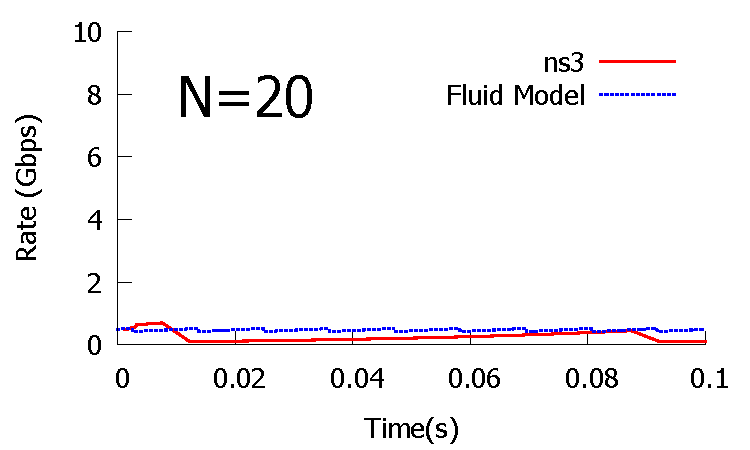
\includegraphics[width=0.45\columnwidth]{figures/timely_validation_20_rate.pdf}
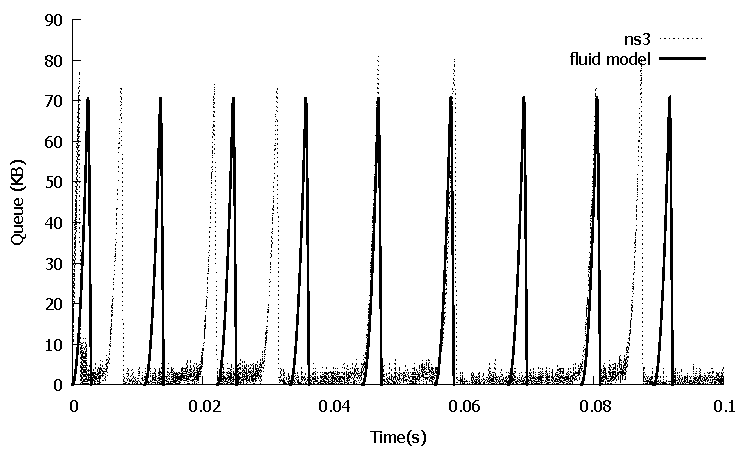
\includegraphics[width=0.45\columnwidth]{figures/timely_validation_20_q.pdf}
}
\caption{Comparison of TIMELY fluid model and simulations}
\label{fig:timely_model_validation}
\end{figure}


\subsection {Analysis}

%\subsubsection{TIMELY has no fixed point, is inherently unstable with unpredictable fairness}
We now show that the TIMELY, as described
in Algorithm~\ref{fig:timely_algo} has \emph{no fixed point}. The implication
is that the queue length never converges, nor do the sending rates of the flows.
The system operates in limit cycles, always oscillating. Moreover, while the
system is oscillating, there are \emph{infinite} solutions for the sending rates
of the flows that satisfy the fluid equations at any point. So, even if we can
limit the magnitude of the limit cycles by choosing parameters carefully, we can
make no claims on the fairness of the protocol since the system could be
operating at any of those infinite solutions.

\begin{thm}[No fixed point for TIMELY] 
\label{thm:nofixed}
The system described in Figure~(\ref{fig:timely_model}), has no fixed points.
\end{thm}
\begin{proof}
We prove the result by contradiction. At the fixed point, all
differential equations converge to 0. Thus:
\begin{equation}
\small
{dq}/{dt} = 0 \; \; \mbox{and} \; \;  \sum_{i} R_i(t) =  C
\end{equation} 
Now, either $g_i > 0$ or $g_i  \le 0$. If $g_i \ne 0$, then:
\begin{equation}
\small
\frac{{dg_i}}{{dt}} =  \frac{\alpha }{{\tau_i^*}}( - g_i(t) + \frac{{q(t
                        - \tau ') - q(t - \tau ' - \tau_i^*
                        )}}{{C*{D_{\min RTT}}}})\\
 =   -\frac{\alpha }{{\tau_i^*}} g_i(t)  \ne  0
\end{equation}
Thus, $g_i$ is zero for $dg_i/dt$ to be zero. But then:
\begin{equation}
\small
{dR_i}/{dt} =  {\delta }/{{\tau_i^*}} \ne 0
\end{equation}
Thus, all derivatives cannot be simultaneously 0 and thus the system has no fixed
point.
\end{proof}

If we modify the fluid model very slightly, by moving the equality condition to
the term involving $g_i$, we get:
\begin{equation}
\small
\frac{{dR_i}}{{dt}} = \left\{ \begin{array}{ll}
\frac{\delta }{{\tau_i^*}}, & q(t - \tau ') < C*{T_{low}}\\
\frac{\delta }{{\tau_i^*}}, & g_i < 0\\
 - \frac{{g_i\beta }}{{\tau_i^*}}R(t), & g_i \ge 0\\
 - \frac{\beta }{{\tau_i^*}}(1 - \frac{{C*{T_{high}}}}{{q(t - \tau ')}})R(t), & q(t - \tau ') > C*{T_{high}}
\end{array} \right.\\
\label{eq:timely_r_modified}
\end{equation}

\begin{figure*}[t]
\center
\subfigure[Both flows start at time 0 at 5Gbps] { 
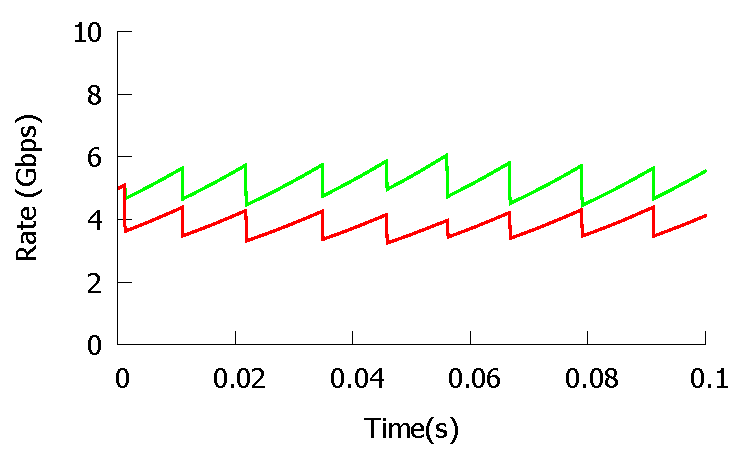
\includegraphics[width=0.3\textwidth]{figures/timely_stability_2f55.pdf}
\label{fig:ts2f55}
}
\subfigure[Both start at 5Gbps, one starts 10ms late] { 
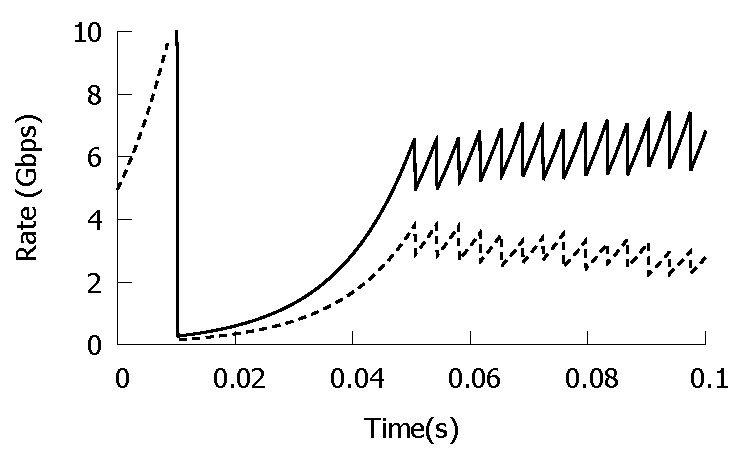
\includegraphics[width=0.3\textwidth]{figures/timely_stability_2ftime.pdf}
\label{fig:ts2f55time}
}
\subfigure[One starts at 7Gbps, the other at 3Gbps] { 
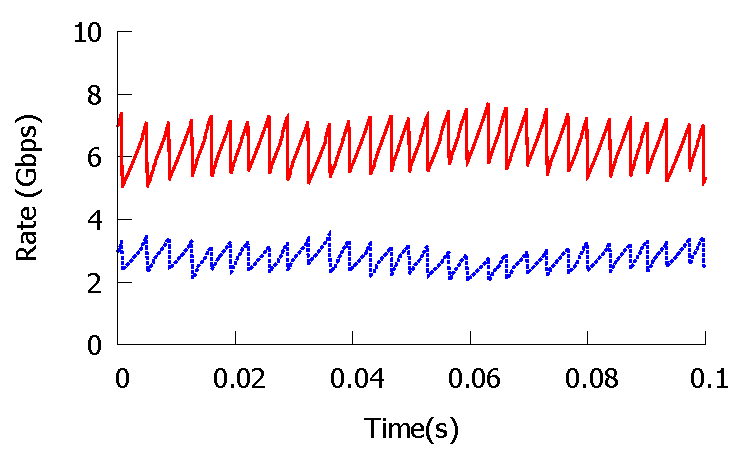
\includegraphics[width=0.3\textwidth]{figures/timely_stability_2f73.pdf}
\label{fig:ts2f73}
}
\vspace{-1em}
\caption{Performance of two TIMELY flows under different starting conditions}
\label{fig:timely_unstable}
\vspace{-1em}
\end{figure*}

This is equivalent to changing the $\le$ sign on line 9 of
Algorithm~\ref{fig:timely_algo} to $<$. This makes little difference in
practice, since floating point computations for $g_i$ rarely yield an exact zero
value -- we have verified this via simulations. With this modification, we can
obtain the condition that with $g_i =0$, $\tfrac{dq}{dt} = 0$, $\tfrac{dg_i}{dt} =
0$ and $C*T_{low} < q < C*T_{high}$. However, now we run into the issue that
TIMELY moves from zero fixed points to \emph{infinite} fixed points!

\begin{thm}[Infinite fixed points]
The system described by Figure~(\ref{fig:timely_model}), with
modification introduced in Equation~\ref{eq:timely_r_modified} has
infinite fixed points
\end{thm}
\begin{proof}
To obtain ${dg_i}/{dt} =0$, we need $g_i = 0$ and ${dq}/{dt} = 0$.  Note that $q$
cannot converge to a value outside of the thresholds $ C*{T_{low}}$ and
$C*{T_{high}}$ as that would imply ${dR_i}/{dt} \ne 0$.

Any value of $q$ such that $C*T_{low} < q < C*T_{high}$ makes ${dR_i}/{dt} = 0$
for any value of $R_i$ as long as $\sum_{i} R_i(t) =  C$ and hence $q$
and $R_i$ have
infinitely many fixed points. 
\end{proof}

There is no requirement that at the fixed point $R_i = {C}/{N}$. In fact,
${R_{i}}/{R_{j}}, i \ne j$ is not even bounded, so we cannot make any
claims on the fairness of TIMELY. Thus the fixed point of TIMELY is entirely
unpredictable. This is borne out by the simulation results shown in
Figure~\ref{fig:timely_unstable}, where we only change the start time and
initial rates of two flows, keeping everything else constant, and we end up in
completely different operating regimes.

\para{Impact of per-burst pacing:}
This analysis begs the question -- why does TIMELY work well in practice, as
reported in~\cite{timely}? The answer appears to lie in the fact that the TIMELY
implementation does not use hardware rate limiters.  Instead, the TIMELY
implementation controls rate by adjusting delay between successive transmissions
of chunks that can be as large as 64KB. Each chunk is sent out at or near line rate.

The results shown in Figure~\ref{fig:timely_unstable} were obtained with
per-packet pacing. If, instead we user per-burst pacing, TIMELY appears to
converge, as shown in Figure~\ref{fig:timely_burst_73_16}. The bursts introduce
enough ``noise'' to de-correlate the flows, and this appears to lead the system
to a relatively stable fixed point. We attempted to mathematically prove that
per-burst pacing would lead to a unique fixed point, but were unable to do so.

In any case, per-burst pacing is not ideal, since it can lead to large
oscillations in queue length, leading to poor utilization. This is apparent in
Figure~\ref{fig:timely_burst_55_64}, where we use 64KB chunks. The initial
chunks sent by the two senders arrive at the switch near-simultaneously (i.e.
``incast''), and both flows receive a very large RTT sample. This causes TIMELY
to reduce its rate drastically (line 8 in the TIMELY algorithm). Since the
subsequent rate increase occurs in small steps ($\delta = 10Mbps$, see line
6.)\footnote{HAI kicks in only after $RTT > T_{low}$. See Algorithm 1 in \cite{timely}}, it takes a long time for the flow rates to climb back to their fair
share. 

These problems can be mitigated to some extent by sending bursts at less than
line rate\footnote{Indeed, the TIMELY does this, see \S~5
in~\cite{timely}.}, by adjusting the burst size, or by adjusting the $T_{min}$
threshold. However, such tuning is fragile, since the right values of these
parameters depend not just on the link speed, but also on the number of
competing flows, which is unknown at the time of configuration. 

In summary, while burst pacing can lead to a fixed point by introducing noise,
it can lead to other problems. The fact that TIMELY cannot
maintain a stable queue length has a detrimental impact on the flow level
performance ({\em e.g.,} flow completion times), especially at higher percentiles.
We illustrate this in Section~\ref{sec:fct}.


Rather than rely on ``noise'' to ensure
convergence and stability, we propose a simple fix to the TIMELY algorithm.

\begin{figure*}[t]
\centering
\mbox{
\begin{minipage}{0.62\textwidth}
\subfigure[Two flows starting at 7 and 3Gbps, 16KB burst] { 
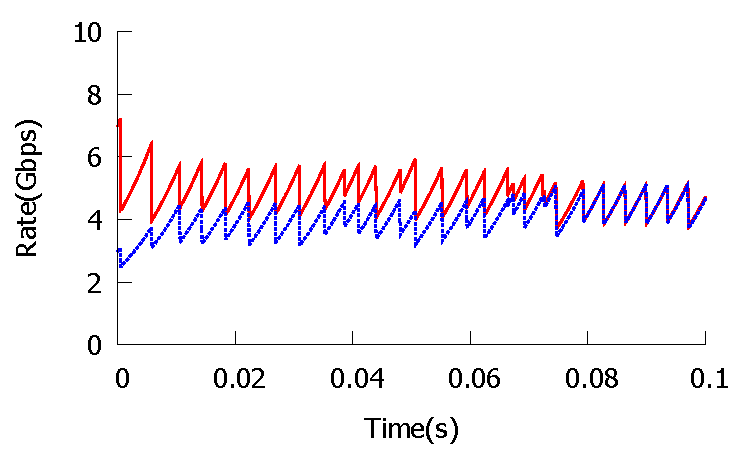
\includegraphics[width=0.47\textwidth]{figures/2f73burst16.pdf}
\label{fig:timely_burst_73_16}
}
\subfigure[Two flows starting at 5Gbps, 64KB burst] { 
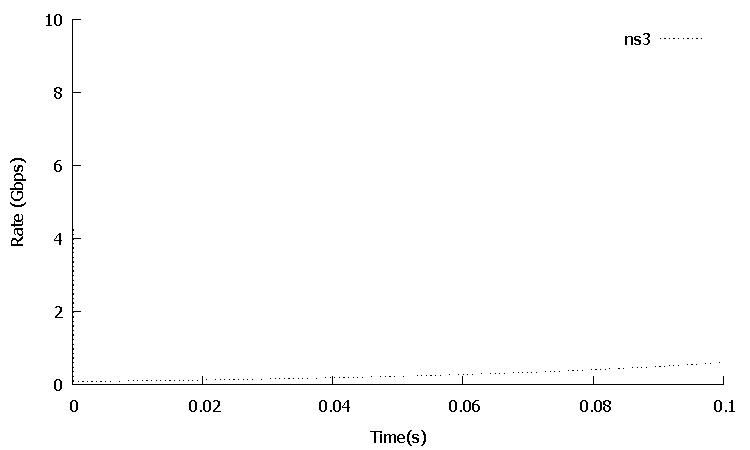
\includegraphics[width=0.47\textwidth]{figures/timely_bursty_64_rate.pdf}
\label{fig:timely_burst_55_64}
}
\vspace{-1em}
\caption{TIMELY with bursts}
\label{fig:timely_sim_bursty}
\end{minipage}
\begin{minipage}{0.36\textwidth}
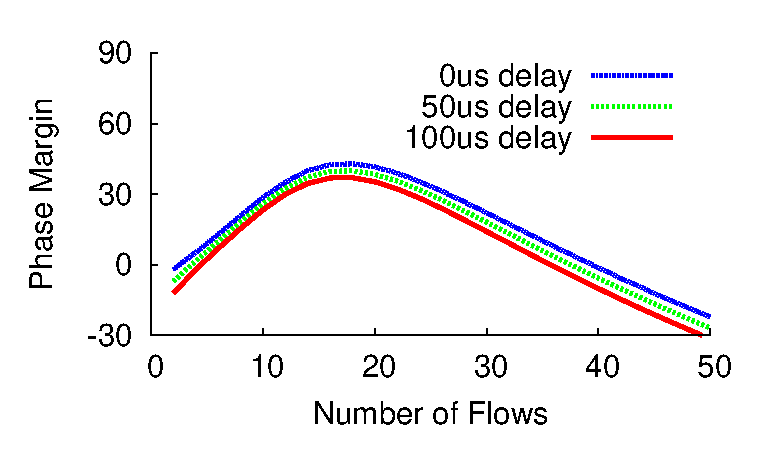
\includegraphics[width=0.99\textwidth]{figures/timely_stability.eps}
\caption{Patched TIMELY stability}
\label{fig:timely_stability}
\end{minipage}
}
\end{figure*}

\subsubsection{Need for hardware rate limiters}

The ns3 simulations shown in Figure~\ref{fig:timely_model_validation} differ
from the TIMELY implementation in one important aspect. The simulator controls
rate by adjusting delay between individual packets. However, doing so in the
real world would require hardware rate limiters. As an engineering compromised
(i.e. to avoid the dependence on hardware rate limiters), the TIMELY
implementation controls rate by adjusting delay between successive transmissions
of chunks that can be as large as 64KB. Each chunk is sent out at line rate.  In
Figure~\ref{fig:timely_sim_bursty} we simulate this bursty behavior for two
flows, for chunk sizes of 16KB and 64KB.

These results clearly demonstrate that TIMELY behaves poorly with larger chunk
sizes. The initial chunks sent by the two senders arrive at the switch
near-simultaneously (i.e. ``incast''), and both flows receive a very large RTT
sample. This causes TIMELY to reduce its rate drastically (line 8 in the TIMELY
algorithm). Since the subsequent rate increase occurs in small steps ($\delta =
10Mbps$, see line 6.), it takes a long time for the flow rates to climb back to
their fair share.

Needless to say, the equations in Figure~\ref{fig:timely_model} model the
``ideal'' TIMELY behavior (infinitely small chunk size) -- and the actual
behavior will approach the ideal one as chunk size is reduced (see results for
16KB chunk size).

\begin{figure}[t]
\center
\subfigure[N=2, 16KB chunk] { 
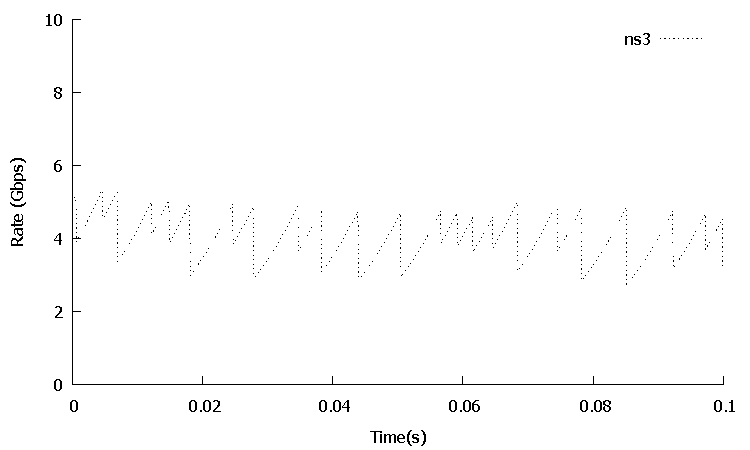
\includegraphics[width=0.4\columnwidth]{figures/timely_bursty_16_rate.pdf}
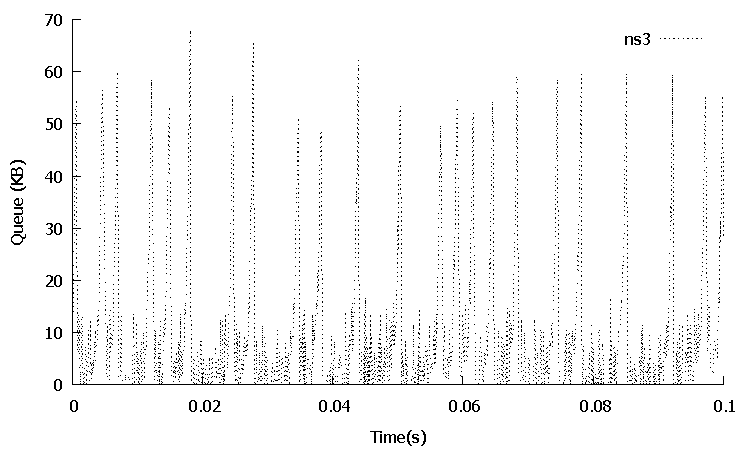
\includegraphics[width=0.4\columnwidth]{figures/timely_bursty_16_q.pdf}
}
\subfigure[N=2, 64KB chunk] { 
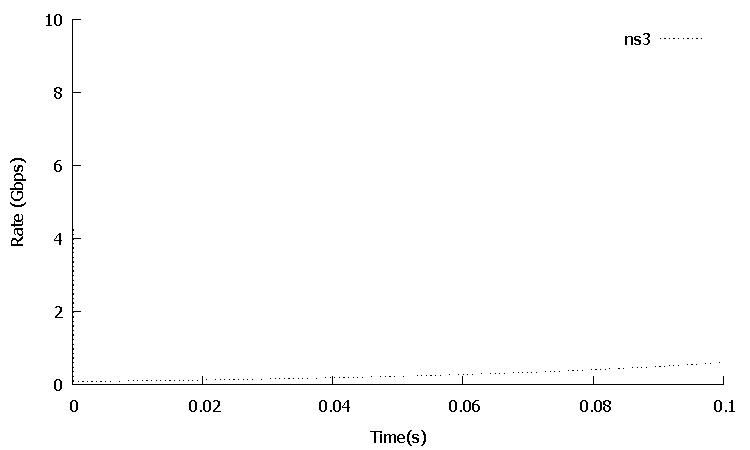
\includegraphics[width=0.4\columnwidth]{figures/timely_bursty_64_rate.pdf}
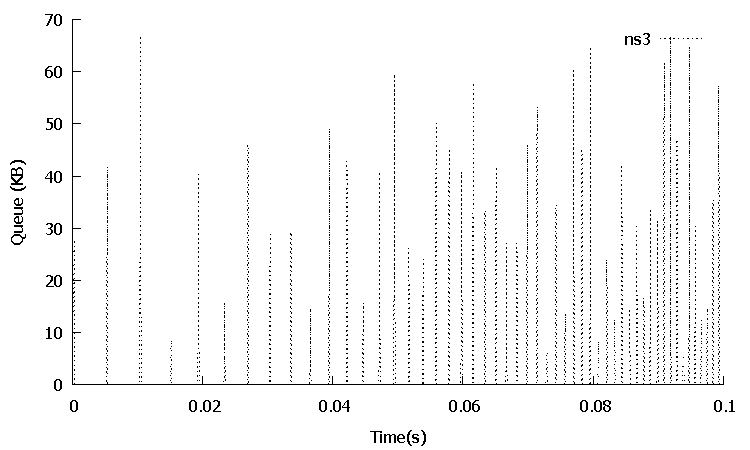
\includegraphics[width=0.4\columnwidth]{figures/timely_bursty_64_q.pdf}
}
\caption{TIMELY with chunk-based rate limiting}
\label{fig:timely_sim_bursty}
\end{figure}

\subsection {Patched TIMELY}
\label{sec:timely_fixed}
%\begin{figure}[t]
%\center
%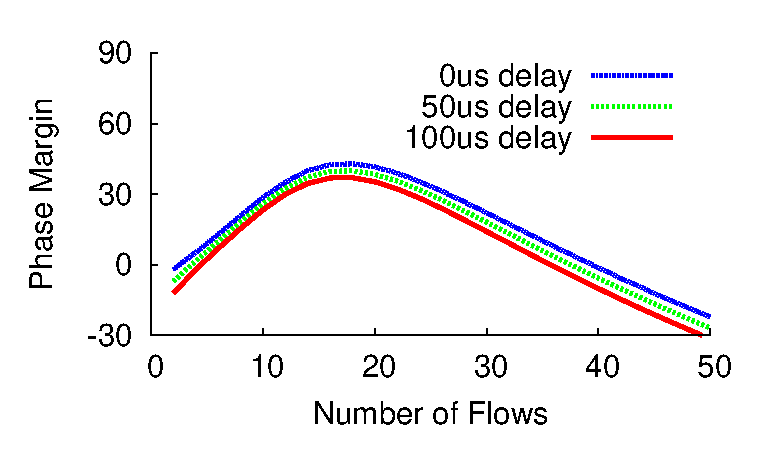
\includegraphics[width=0.33\textwidth]{figures/timely_stability.eps}
%\caption{Patched TIMELY stability}
%\label{fig:timely_stability}
%\end{figure}

\begin{figure*}[t]
\center
\subfigure[Two flows, 7Gbps and 3Gbps] { 
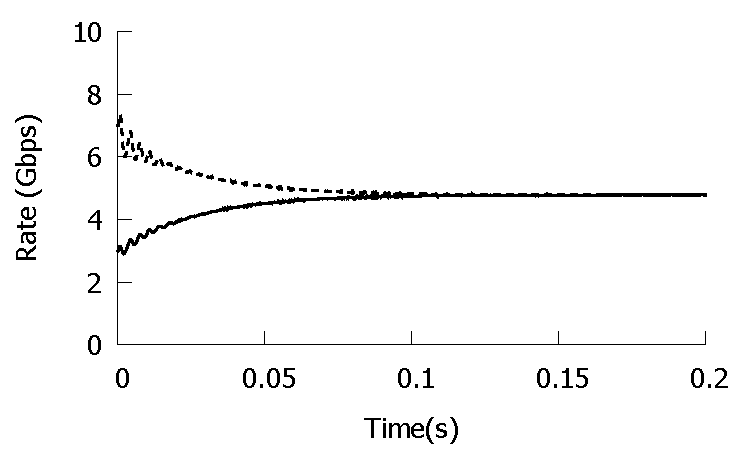
\includegraphics[width=0.3\textwidth]{figures/timely_stability_2f73_fixed.pdf}
\label{fig:timely_fixed_a}
}
\subfigure[Two flows, 7Gbps and 3Gbps] { 
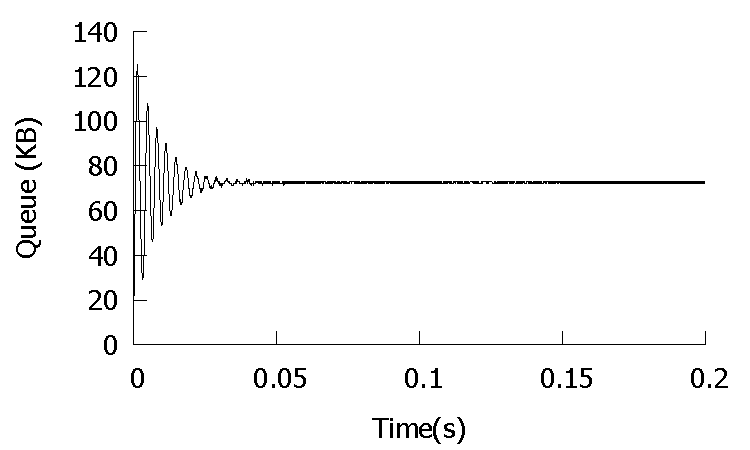
\includegraphics[width=0.3\textwidth]{figures/timely_stability_q_2f73_fixed.pdf}
\label{fig:timely_fixed_b}
}
\subfigure[40 flows, starting at 0.25Gbps] { 
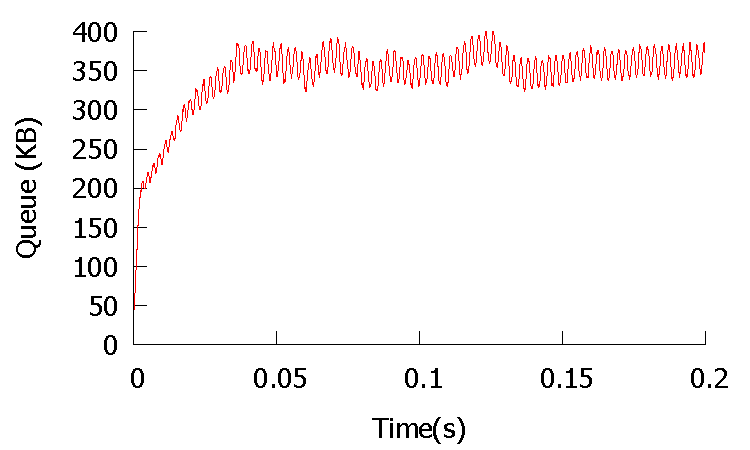
\includegraphics[width=0.3\textwidth]{figures/timely_stability_q_40f_fixed.pdf}
\label{fig:timely_fixed_c}
}
\vspace{-0.5em}
\caption{Performance of patched TIMELY}
\vspace{-0.5em}
\label{fig:timely_fixed}
\end{figure*}

In order to ensure there is a unique fixed point, and all flows get fair
share and are stable at the fixed point, we make two minor modifications over
TIMELY, as shown in Algorithm~\ref{fig:timely_fixed_algo}. We only modify the
last four lines of Algorithm~\ref{fig:timely_algo}.

\begin{algorithm}[t]
\footnotesize
{
\begin{algorithmic}[1]
%\Procedure{CalcRate}{$newRTT$}
\State $newRTTDiff \gets newRTT - prevRTT$
\State $prevRTT \gets newRTT$
\State $rttDiff \gets (1-\alpha) \cdot rttDiff + \alpha \cdot newRTTDiff$
\State $rttGradient = rttDiff/D_{minRTT}$
\If {$newRTT < T_{low}$}
        \State $rate \gets rate + \delta$
\ElsIf {$newRTT > T_{high}$}
        \State $rate \gets rate \cdot  (1 - \beta \cdot (1 - T_{high}/newRTT))$
\Else
		\State $weight \gets w(rttGradient)$	
		\State $error \gets \frac{{newRTT - RT{T_{ref}}}}{{RT{T_{ref}}}}$
        \State $rate \gets \delta (1-weight) +  rate \cdot (1 - \beta \cdot weight  \cdot error)$
\EndIf 
%\EndProcedure
\end{algorithmic}
}
\caption{Patched TIMELY rate calculation}
\label{fig:timely_fixed_algo}
\end{algorithm}

First, we make the step of rate decrease rely on absolute RTT, instead of the
gradient of RTT. In effect, this means that all flows have the knowledge of the
bottleneck queue length.  This ensures two things. First, the system can have a
unique fixed point, determined by the RTT\footnote{Recall that the issue with
the original TIMELY was that the RTT gradient could be the same, but absolute
RTTs could be different}.  Second, all flow can converge to the same rate, since
they share the knowledge of the bottleneck RTT.  The side effect, of course, is
that, with different number of flows, the fixed point of queue can be different.
We will address this in \S\ref{sec:discuss}. 

Second, we use a continuous weighting function $w(g)$ to make the transition
between rate increase and rate decrease smooth. This avoids the on-off behavior
that causes oscillation.  This is similar to the fact that probabilistic ECN
marking stabilizes TCP~\cite{misra2000fluid}, DCTCP~\cite{dctcp-analysis},
QCN~\cite{qcn-analysis} and DCQCN. With $w(g)$, we combine the two conditions of
$g \le 0$ and $g>0$ in the $dR(t)/dt$ equation:
\begin{equation}
\small
\frac{{dR_i}}{{dt}} = \left\{ \begin{array}{ll}
\frac{\delta }{{\tau *}}, & q(t - \tau ') < C*{T_{low}}\\
\frac{{(1 - {w_i})\delta }}{{\tau *}} - \frac{{{w_i}\beta {R_i}(t)}}{{\tau *}}\frac{{q(t - \tau ') - q'}}{{q'}}, & Otherwise\\
 - \frac{\beta }{{\tau *}}(1 - \frac{{C*{T_{high}}}}{{q(t - \tau ')}})R_i(t), & q(t - \tau ') > C*{T_{high}}
\end{array} \right.\\
\label{eq:timely_fixed}
\end{equation}
where $w_i$, the weight of rate decreasing, is a function of $g_i$, and must satisfy $0 \le w_i(g_i) \le 1$ for any $g$. 
Intuitively, $w_i(g_i)$ is monotonically increasing with $g_i$, because larger RTT gradient should lead to larger 
rate decrease. In original TIMELY protocol, $w_i(g_i)$ is an indicator function of $g_i$, {\em i.e.,} 
$w_i(g_i)=1$ when $g \le 0$, and $w_i(g_i)=0$ when $g<0$. Here we simply use a linear function of $g_i$ for $w_i$:
\begin{equation}
\small
{w_i} = \left\{ \begin{array}{ll}
0, & {g_i \le  - \frac{1}{4}} \\
2{g_i} + \frac{1}{2}, & { - \frac{1}{4} < g_i < \frac{1}{4}} \\
1, & {g_i \ge \frac{1}{4}}
\end{array} \right.
\end{equation}
In Equation~\ref{eq:timely_fixed}, $q'$ is a reference queue length. We simply set it as $C*T_{low}$, 
so that we decrease the rate faster if the queue length exceeds $C*T_{low}$. All
other TIMELY parameters remain the same except we set $\beta=0.008$ and $Seg=16KB$. 
We prove that this patched TIMELY protocol has desirable stability and convergence properties
that original TIMELY does not guarantee:


\begin{thm}[Patched TIMELY's fixed point.]
The system described in Equation~\ref{eq:timely_fixed} has a unique fixed point.
All flows have the same rate at this fixed point, and the queue length is:
\begin{equation}
\small
{q^*} = \frac{{N{R_{AI}}q'}}{{\beta C}} + q'
\label{eq:timely_fixed_q}
\end{equation}
The system described in Equation~\ref{eq:timely_fixed} always exponentially converges to 
the unique  fixed point.
\end{thm}

The detailed proof is omitted and can be found at~\cite{patchedtimelyproof}.



\if 0
\begin{proof}
Let the LHS of Equation~\ref{eq:timely_g} be 0, and $q(t - \tau ') - q(t - \tau ' - \tau *) = 0$ at the fixed 
point, we know $g_i^*=0$. Thus, $w_i^*=0.5$. Let the LHS of Equation~\ref{eq:timely_fixed} be 0. Because
all flows share the same queue length $q^*$, we have:
\begin{equation}
\small
R_1^* = R_2^* = ... = R_N^*
\end{equation}
The sum of all flow rates must be $C$ at the fixed point, therefore each flow has fair share $C/N$. 
\end{proof}
In addition, we can easily obtain the fixed point of queue length, which depends on $N$, the number of flows:
\begin{equation}
\small
{q^*} = \frac{{N{R_{AI}}q'}}{{\beta C}} + q'
\label{eq:timely_fixed_q}
\end{equation}

\begin{thm}[Patched TIMELY convergence.]
The system described in Equation~\ref{eq:timely_fixed} always converges to the unique fixed point.
\end{thm}
\begin{proof}
Here we provide a brief proof. First, the queue length $q$ always
converges to the fixed point $q^*$. This can be proved by contradiction because whenever $q$ stabilizes
at $q>q^*$, we have ${\left. {\frac{{dR}}{{dt}}} \right|_{q > {q^*}}} < {\left. {\frac{{dR}}{{dt}}} \right|_{q = {q^*}}} = 0$, 
leading to queue length decrease. The case of $q<q^*$ is similar. 

Second, once queue length converges to a stable state, we see that $g_i$ converges to 0.
We denote ${g_i}(n)$ as the value of $g_i$ upon the completion of $n$th segment after queue
length converges:
%Equation~\ref{eq:timely_g} becomes
%$\frac{{d{g_i}}}{{dt}} =  - \frac{\alpha }{{{\tau_i^*}}}{g_i}$. By turning it into a discrete model
%with $\tau_i^*(t)$ as intervals, we see that $g_i$ converges to 0:
\begin{equation}
\small
\left| {{g_i}(n + 1)} \right| = \left( {1 - \alpha} \right)\left| {{g_i}(n)} \right| = {\left( {1 - \alpha} \right)}^{n+1} \left| {{g_i}(0)} \right|
\end{equation}
Finally, after $g_i$ converges to 0, which means $w_i=0.5$, we rewrite the $j$th flow's Equation~\ref{eq:timely_fixed} 
and subtract it from $i$th flow's. Without losing generality, we choose $i,j, s.t.$ $i$th flow is the fastest among all flows,
whereas $j$th flow is the slowest. After simplification, we get:
\begin{equation}
\small
\frac{{d\left( {{R_i} - {R_j}} \right)}}{{dt}} = \frac{\delta }{{2Seg}}\left( {1 - \frac{N}{C}\left( {{R_i} + {R_j}} \right)} \right)\left( {{R_i} - {R_j}} \right)
\end{equation}
Among the total $N$ flows, there must exist at least one flow not slower than the fair share $C/N$.
Therefore, ${{R_i} + {R_j}} > C/N$ since $R_i$, the fastest flow, is not slower than $C/N$.
Solving the differential equation with ${{R_i} - {R_j}}$ as the variable, we get that the rate 
difference between the fastest and slowest flow decreases over time exponentially, as we shall see below. 

\para{Exponential convergence.} We estimate the TIMELY convergence time {\em after}
the queue stabilizes. We start from the case of $N=2$, where $R_i + R_j = C$
because of Equation~\ref{eq:timely_q}.
Then we get:
\begin{equation}
\small
{R_i}(t) - {R_j}(t) = \left( {{R_i}(0) - {R_j}(0)} \right){e^{\frac{{\delta (1 - N)}}{{2Seg}}t}}
\end{equation}
Once the fastest flow and slowest flow converge to the same rate, all flow rates converge to the unique fixed point.
\end{proof}

We use the same definition of ``converged'' as in
\S~\ref{sec:dcqcn_convergence}. Thus, the convergence
time is the smallest $t$ that satisfies (assuming two flows start with maximum possible rate difference, $C$):
\begin{equation}
\small
{e^{\frac{{\delta (1 - N)}}{{2Seg}}t}}C \le \frac{{0.1 \times C}}{N}
\label{eq:timely_convergence_time}
\end{equation}
With $N=2$ and parameters we choose earlier, we get $t = 76.7ms$. With (\ref{eq:timely_convergence_time}), 

It is easy to see that
with larger $N$,\footnote{Details omitted.} larger $\delta$ or smaller $Seg$, patched TIMELY will converge faster.

\fi

We verify patched TIMELY convergence and stability using simulations.
Figure~\ref{fig:timely_fixed_a} and~\ref{fig:timely_fixed_b}, shows that flows
with different initial rates converge to the fixed point and are stable without
oscillation, opposed to Figure~\ref{fig:ts2f73}. Results for the case depicted
in Figure~\ref{fig:ts2f55time} are similar.

\para{Stability.} We proceed as we did for DCQCN -- linearize the equations,
Laplace transform and compute the phase margin of its characteristic equation.
The phase margin result shows this system is stable until the number of flows is
greater than 40 (Figure~\ref{fig:timely_stability}).  This is again confirmed by
NS-3 simulation (Figure~\ref{fig:timely_fixed_b} and ~\ref{fig:timely_fixed_c}).
After 40 flows, the phase margin falls below 0 rapidly because more flows lead
to larger queue size (see Equation~\ref{eq:timely_fixed_q}), thus leading to
larger feedback delay (see Equation~\ref{eq:timely_taup}).  This leads to system
instability. In general, with some minor tuning, TIMELY can be stable within a
range of number of flows.


% \subsection {Impact on flow completion time}

While stability and fairness are important performance metrics for any
congestion control protocol, the end users often care about flow completion
times, especially for short flows~\cite{rcp}. The fact that TIMELY cannot
maintain a stable queue length has a detrimental impact on flow completion
times, especially at higher percentiles. We illustrate this with a simple
simulation, using the classic dumbbell topology shown in
Figure~\ref{fig:fct_topo}. The topology consists of 20 nodes -- 10 senders and
10 receivers. All traffic flows across the bottleneck link between the two
switches, SW1 and SW2. All links are 10Gbps with 1$\mu$s latency.

The traffic consists  of long and short-lived flows, between pairs of randomly
selected sender and receiver nodes. The flow size distribution is derived from
the traffic distribution reported in~\cite{dctcp}. The interarrival time of
flows is picked from am exponential distribution. The load on the bottleneck
link is varied by changing the mean of the distribution. This traffic generation
model was also used in several recent studies, including pFabric~\cite{pfabric}
and ProjecToR~\cite{projector}. 

Both DCQCN and TIMELY used the default parameter settings recommended
in~\cite{dcqcn} and ~\cite{timely}, respectively. 

The metric of interest is the flow completion time of small flows. Following pFabric~\cite{pfabric}, we define small flows as flows that send fewer than 100KB. Results with other other
thresholds are similar.

Figure~\ref{fig:fct_results} shows the median and 90th percentile of FCT and
DCQCN, TIMELY original and TIMELY (fixed) as the load is varied. TIMELY (fixed) is our modification to TIMELY's protocol to ensure a unique fixed point~\S\ref{sec:timely_fixed}. The X axis shows relative load: load factor of 1 corresponds to an average of 8Gbps of traffic on the bottleneck link. The scaling is linear. We see that at higher loads, FCT for both TIMELY and TIMELY (fixed) is high, and highly variable. The reason is illustrated in detail in Figure~\ref{fig:fct_cdf}, which shows the CDF of the flow completion time for
load factor of 0.8. The reason for TIMELY's poor performance is evident from
Figure~\ref{fig:fct_queue}, which shows the queue length at the link between
SW1 and SW2 for a load factor of 0.8, which shows that queue length under TIMELY
can be high, and highly variable. Note that TIMELY (fixed) is operating in between the original TIMELY protocol and DCQCN. This is because our fix is ensuring a unique fixed point without changing the dynamics of TIMELY's queue build up. 

\begin{figure*}[t]
\centering
\mbox{
\begin{minipage}{0.36\textwidth}
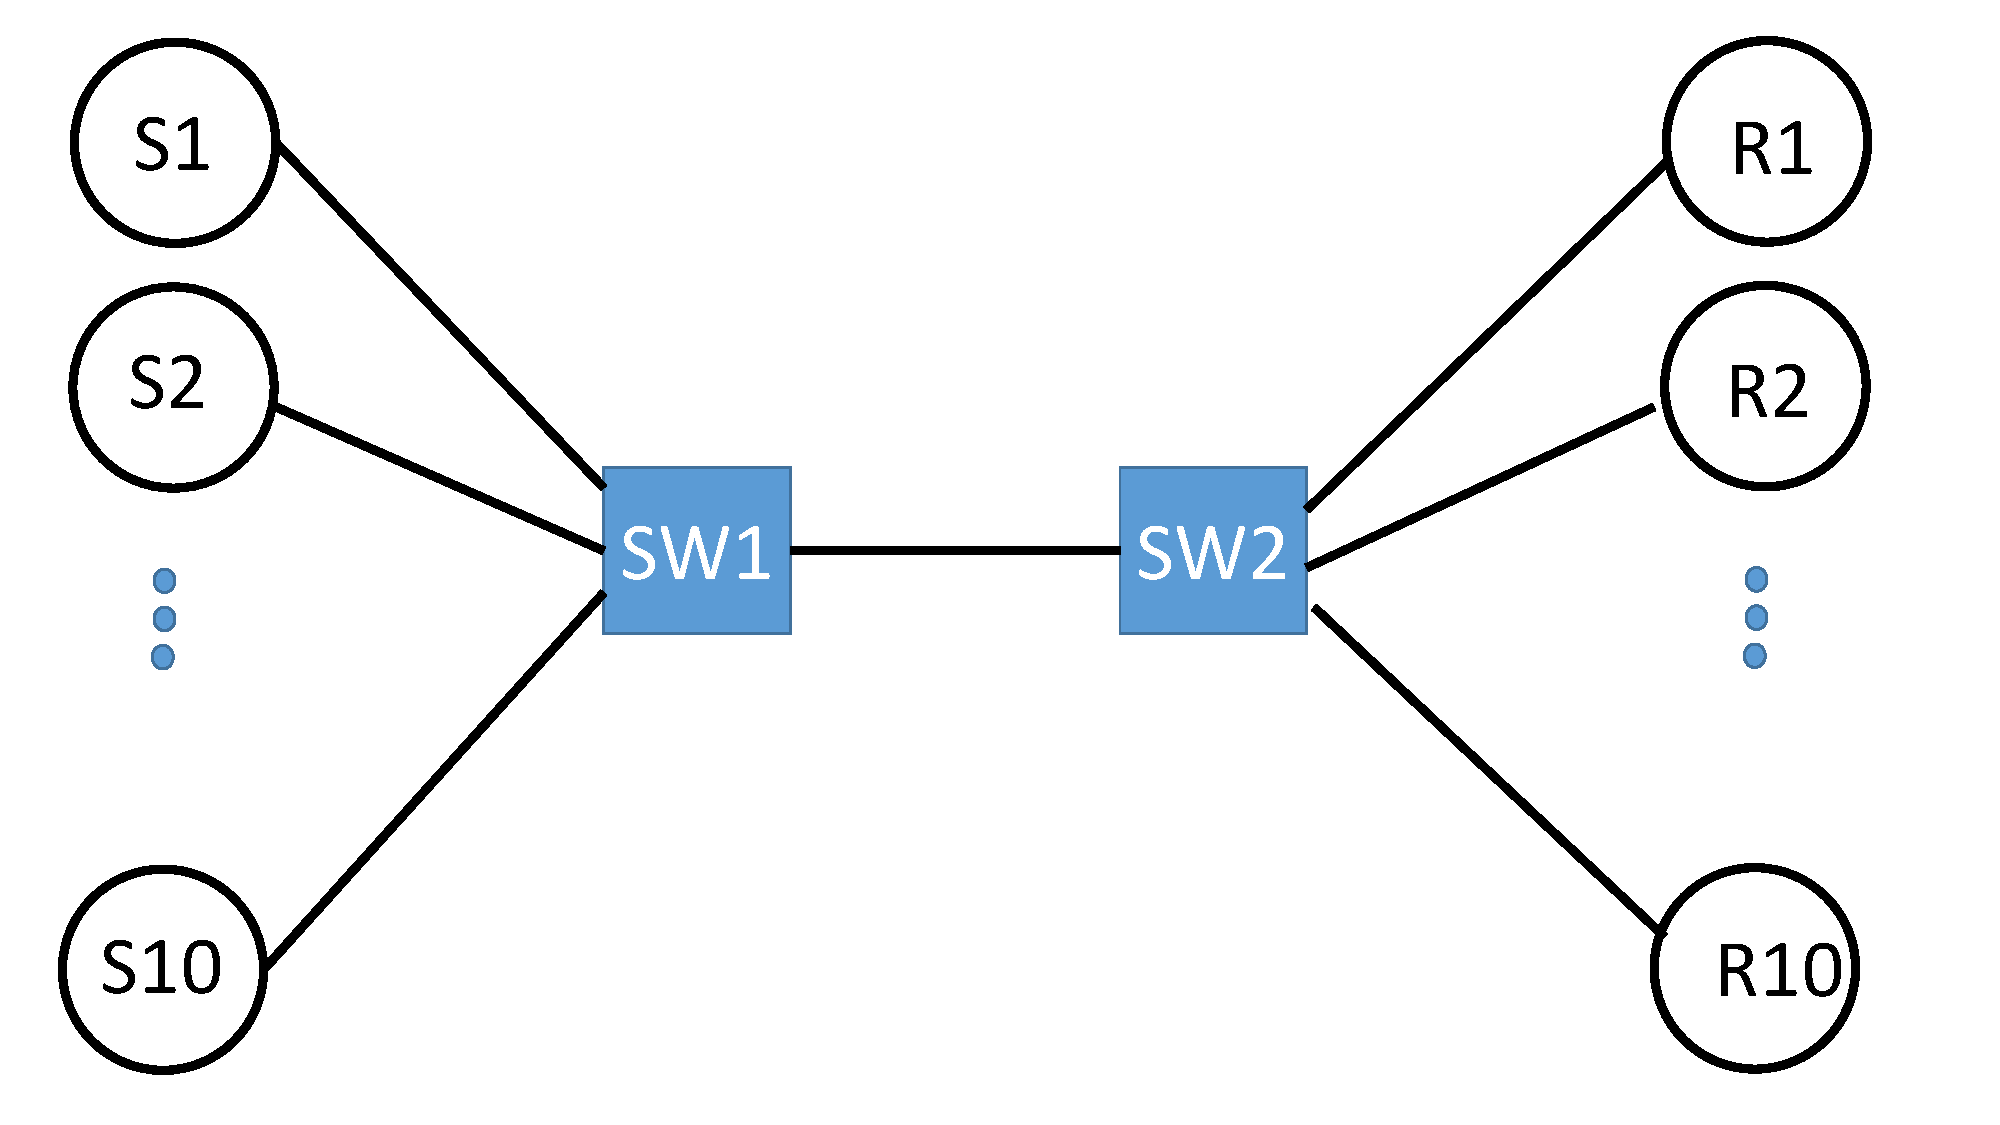
\includegraphics[width=0.99\textwidth]{figures/dumbbell.pdf}
\caption{The dumbbell toplogy. All links are 10Gbps with 1$\mu$s latency.}
\label{fig:fct_topo}
\end{minipage}
\begin{minipage}{0.62\textwidth}
\subfigure []{ 
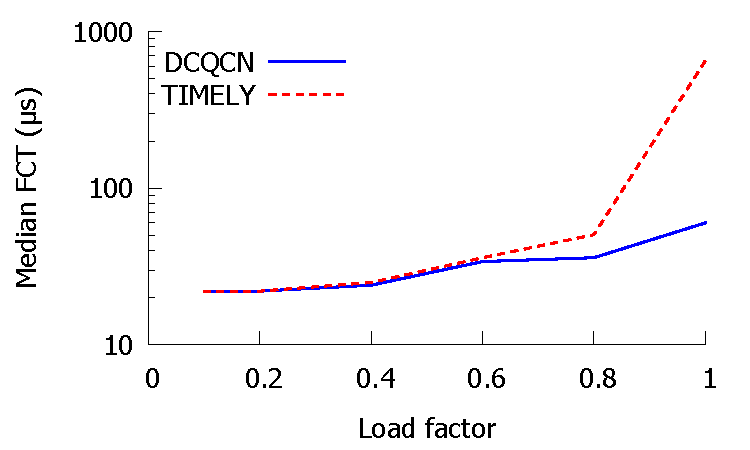
\includegraphics[width=0.48\textwidth]{figures/fct_median.pdf}
\label{fig:fct_median}
}
\subfigure []{ 
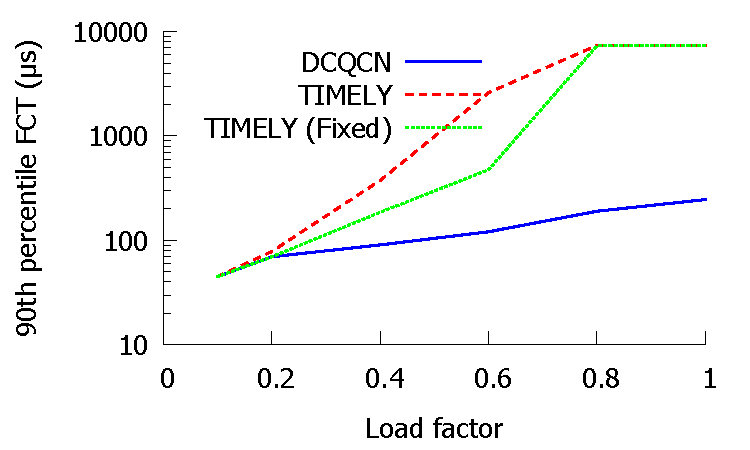
\includegraphics[width=0.48\textwidth]{figures/fct_90.pdf}
\label{fig:fct_90}
}
\caption{Median and 90th percentile of FCT of small flows. Note log scale on Y axis.}
\label{fig:fct_results}
\end{minipage}
}
\end{figure*}

\if 0
\begin{figure}[t]
\center
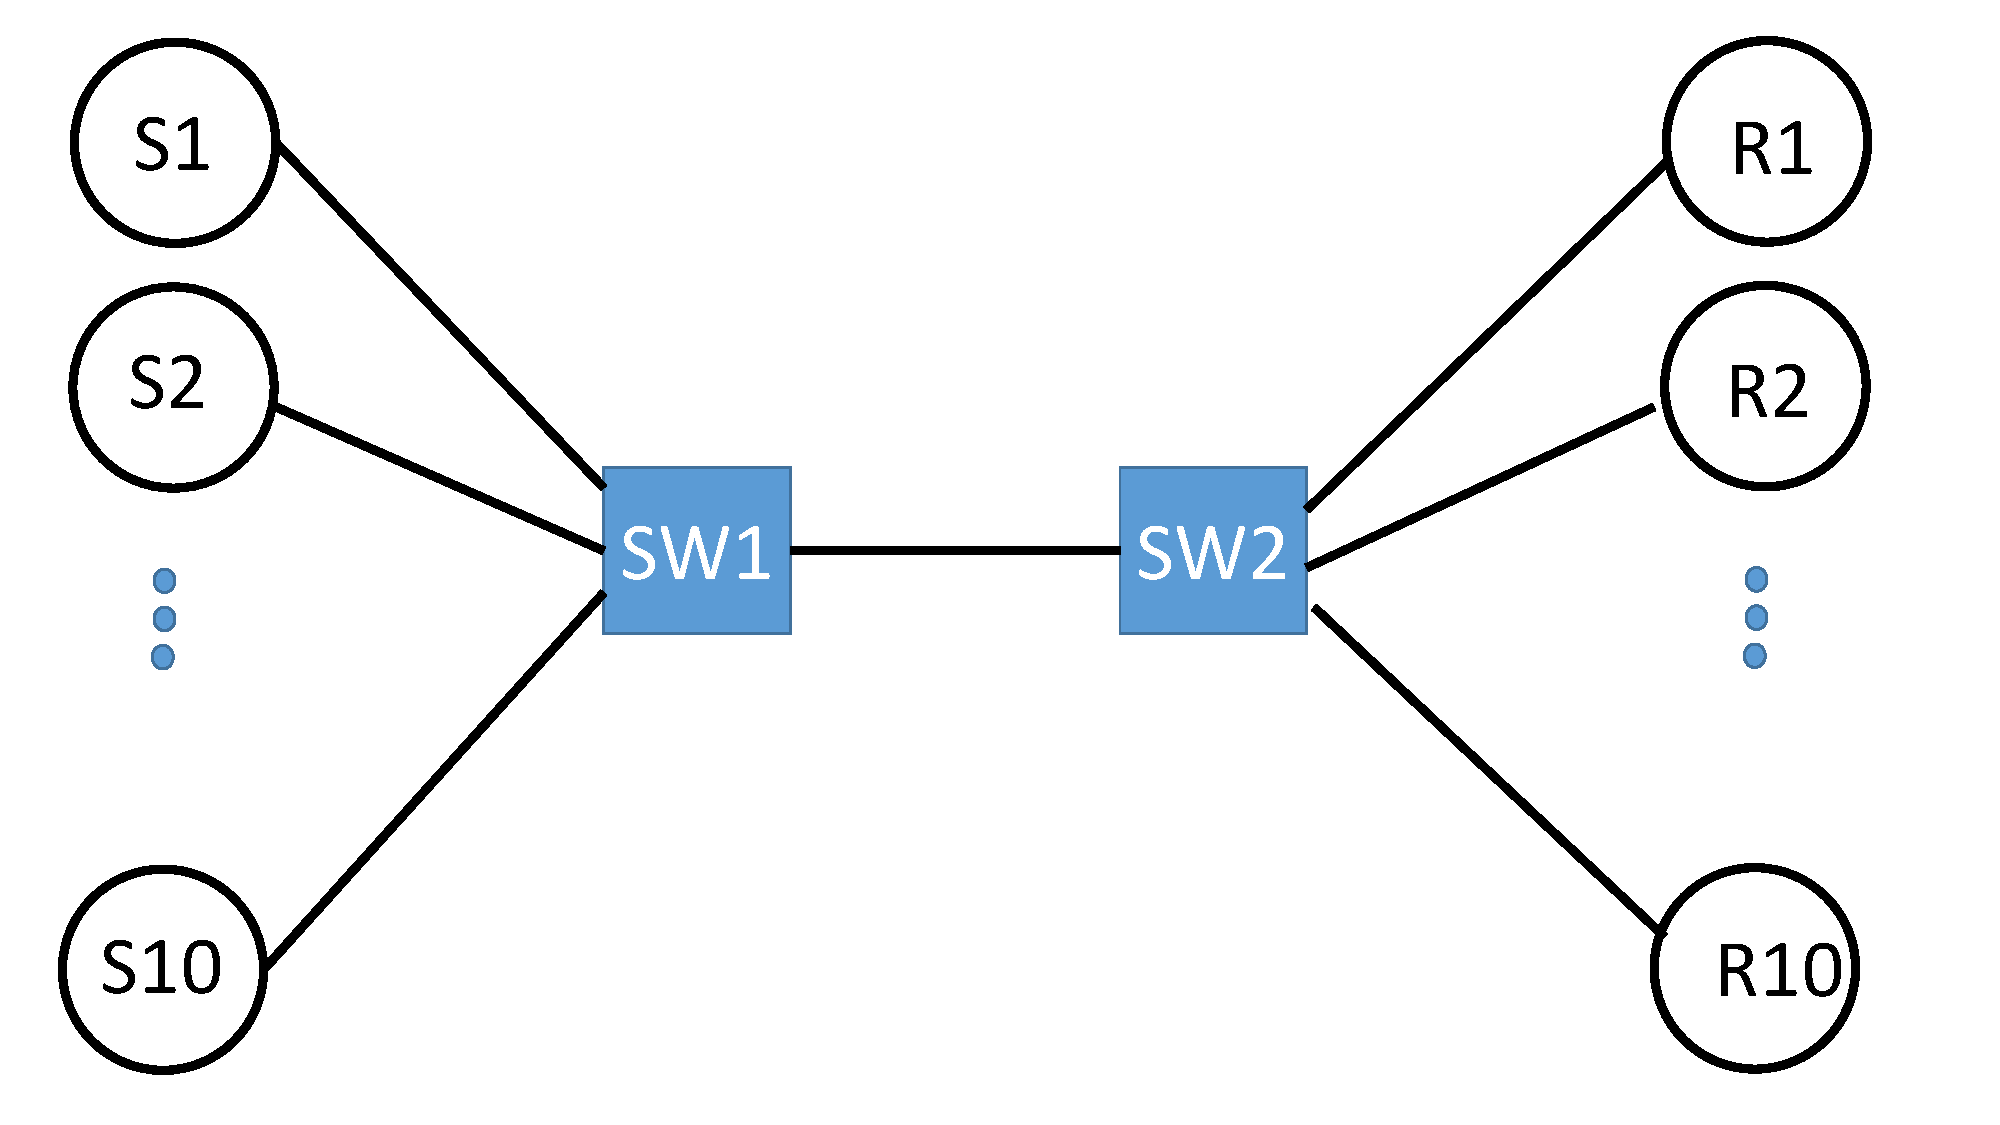
\includegraphics[width=0.3\textwidth]{figures/dumbbell.pdf}
\caption{The dumbbell toplogy. All links are 10Gbps with 1$\mu$s latency.}
\label{fig:fct_topo}
\end{figure}

\begin{figure}[t]
\center
\subfigure []{ 
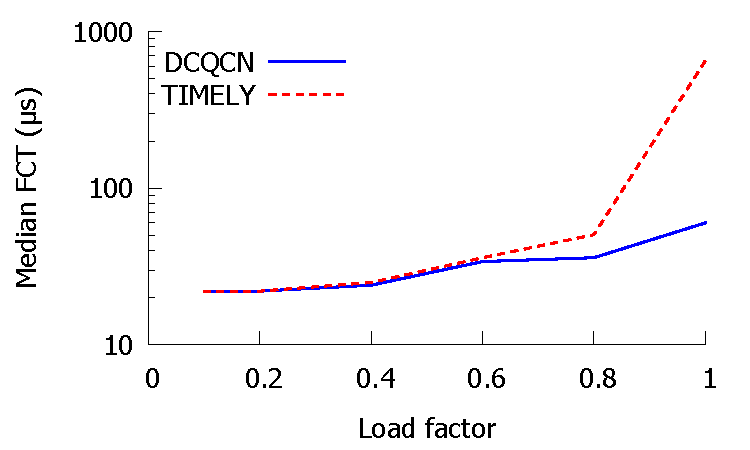
\includegraphics[width=0.3\textwidth]{figures/fct_median.pdf}
\label{fig:fct_median}
}
\subfigure []{ 
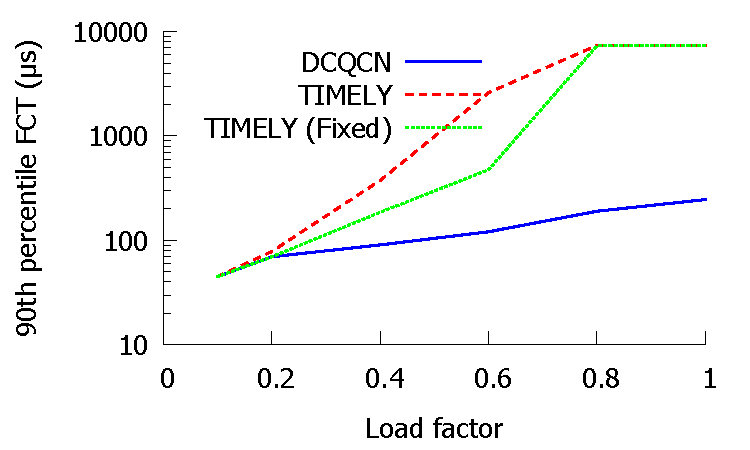
\includegraphics[width=0.3\textwidth]{figures/fct_90.pdf}
\label{fig:fct_90}
}
\caption{Median and 90th percentile of FCT of small flows. Note log scale on Y axis.}
\label{fig:fct_results}
\end{figure}
\fi


\begin{figure*}[t]
\centering
\mbox{
\begin{minipage}{0.32\textwidth}
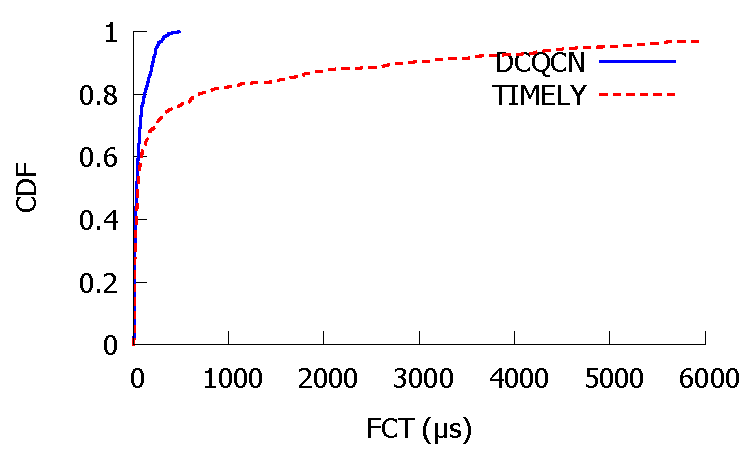
\includegraphics[width=0.99\textwidth]{figures/fct_cdf.pdf}
\caption{CDF of FCT for load=0.8}
\label{fig:fct_cdf}
\end{minipage}
\quad
\begin{minipage}{0.32\textwidth}
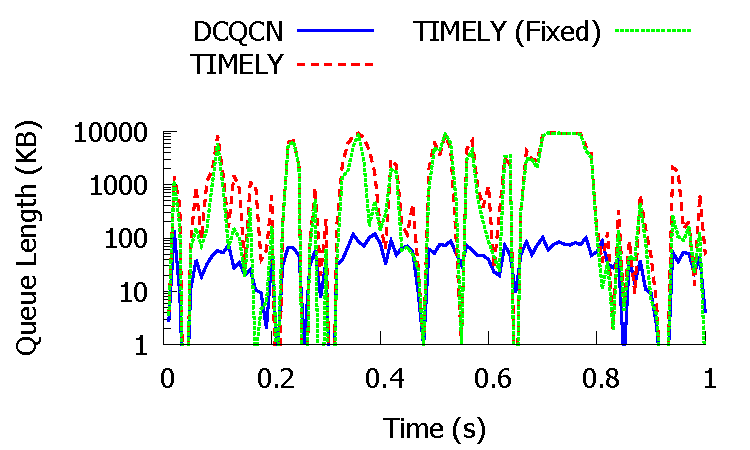
\includegraphics[width=0.99\textwidth]{figures/fct_queue.pdf}
\caption{Bottleneck Queue for load=0.8. Note log scale on Y axis.}
\label{fig:fct_queue}
\end{minipage}
\quad
\begin{minipage}{0.30\textwidth}
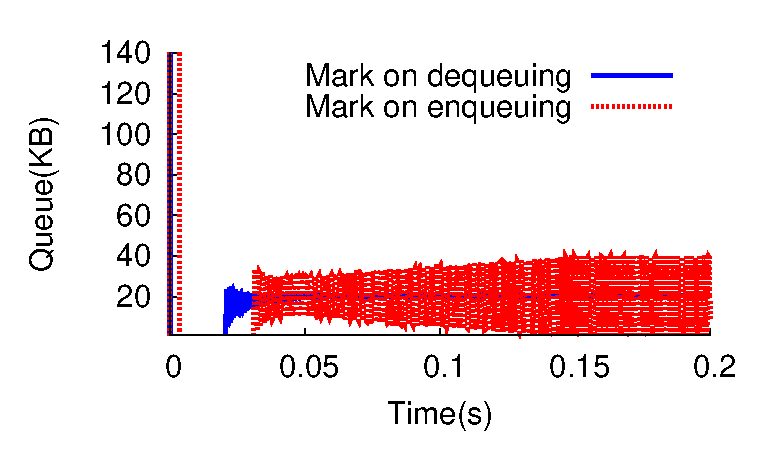
\includegraphics[width=0.99\textwidth]{figures/dcqcn_bufferbloat.eps}
\caption{DCQCN stability when two flows compete for a 40Gbps 
bottleneck with 85$\mu$s feedback delay.}
\vspace{-1.5em}
\label{fig:dcqcn_bufferbloat}
\end{minipage}
}
\end{figure*}

\if 0
\begin{figure}[t]
\center
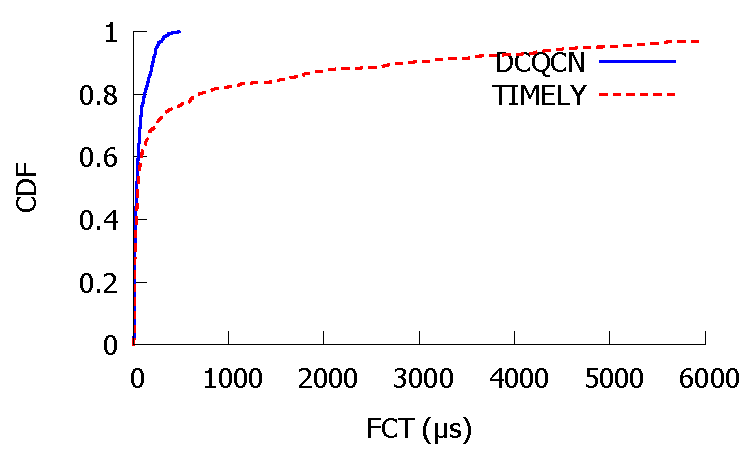
\includegraphics[width=0.3\textwidth]{figures/fct_cdf.pdf}
\caption{CDF of FCT for load=0.8}
\label{fig:fct_cdf}
\end{figure}

\begin{figure}[t]
\center
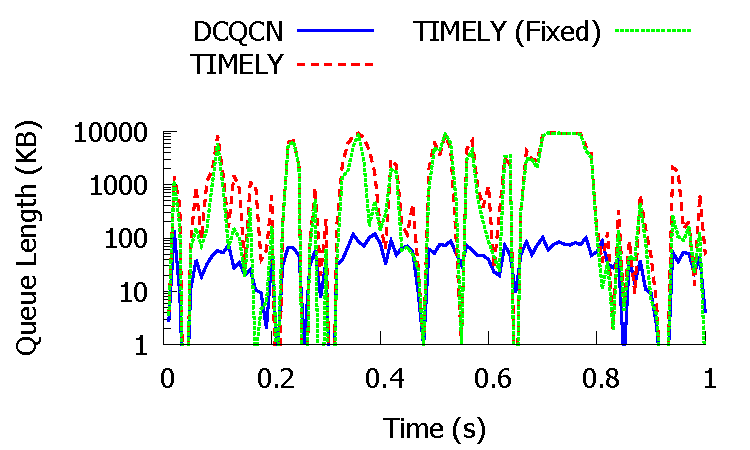
\includegraphics[width=0.3\textwidth]{figures/fct_queue.pdf}
\caption{Bottleneck Queue for load=0.8. Note log scale on Y axis.}
\label{fig:fct_queue}
\end{figure}
\fi

We note that in all cases, the link utilization is roughly the same for DCQCN
and TIMELY, indicating that the long flows performed similarly with both
schemes.

\section{Discussion}

We next prove another result that gives a fundamental tradeoff between
fairness and guaranteed delay for protocols that
rely on delay measurements at the end points to implement congestion
control.
\begin{thm}[Fairness/Delay tradeoff]
For congestion control mechanisms that relay purely on end to end
delay measurements, you can either have fairness or a guaranteed delay
bound, but not both simultaneously.
\end{thm}
\begin{proof}
Suppose you have N flows sharing a link of capacity $C$. Then every flow
should distributedly arrive at a rate $C/N$ and the flows need to know
this $N$. If we use end to end delay as the only signal, then this delay
has to carry information about $N$ and hence the converged delay
depends on $N$ and cannot be guaranteed independently. Conversely, if we implement a guaranteed delay congestion
control scheme at the end points, they
will converge to any rate $R_i$ such that $\sum_{i=0}^{N}R_i = C$
making the derivative of measured delay 0 and the actual delay equal
to the guarantee. Since the guarantee is set independent of $N$, the
actual delay contains no information on N and 
thus such a scheme cannot ensure fairness.
\end{proof}


%%% Local Variables:
%%% mode: latex
%%% TeX-master: "main"
%%% End:

\section {ECN versus Delay}
\label{sec:discuss}
In the previous sections, we saw that barring the small anomaly, DCQCN remains
stable as the number of flows increase. We also saw that this is not the case
for TIMELY. However, for both protocols, the fixed point of the queue
and hence the round trip delay increases with the number of contending
flows, and this makes designing the controller more difficuly with TIMELY as compared to DCQCN.


Let's assume a single-bottleneck scenario, and assume that ECN marking is used
to convey congestion information. Typical shared-buffer switches, especially
those that use Broadcom's merchent sillicon, do ECN marking on {\em packet
egress}. When a packet is ready to depart, the controller checks the egress
queue for that port {\em at that instant}, and depending on the specified
marking algorithm (e.g.  Equation~\ref{eq:mark}), decides whether to mark the
packet. Thus, the mark carried by the packet conveys information about the state
of the queue at the time the packet {\em departs} the queue. In other words,
information carried by just-departed packet (say $p_i$) is influenced by all the
packets that arrived in the queue {\em after} $p_i$ arrived, but before $p_i$
left. 

On the other hand, consider what RTT measurements do. If the egress queue
discipline is FIFO within a priority class, (which it typically is), the delay
experienced by a packet reflects the state of the queue at the time the packet
{\em arrives} at the queue. Subsequent packet arrivals have no bearing on the
delay experienced by the packet. 

This seemingly small detail means that the information about queue state
conveyed by RTT measurements is always {\em stale} compared to what can be
conveyed by ECN markings. In practice, this means that as the queue length
increases, congestion control algorithms that rely on RTT suffer from increasing
{\em lag} in their control loop, making them unstable. Since steady state queue
length typically increases with number of flows, RTT based congestion control is
is more likely to become unstable, compared to ECN-based congestion control.

This issue is critical in data center networks, because queueing delays can
easily dominate switching and propagation delays.  For example, an Arista
7040QX32 has 40Gbps ports, and a total shared buffer of switch has 12MB. Even if
just 1MB worth of queue builds ip at an egress port, it takes 200 $\mu$s to
drain. In contrast, the one-hop propagation delay, with cut-through forwarding
is enabled, are in the range of 1-2 $\mu$s. Typical diameter of a DC network is
6 hops, propagation delay is just 10-18 $\mu$s. In contrast, in wide area
networks, queuing delays and propagation delays can be comparable (excluding
scenarios like buffer bloat~\cite{bufferbloat}). 

However, one can ask the question - can we build congestion control protocols
that are guaranteed to maintain a fixed queue length at the bottleneck,
regardless of the number of flows? The answer, as we show below, turns out to be
yes - but you can guarantee fairness only if you use ECN.

We next prove another result that gives a fundamental tradeoff between fairness
and guaranteed delay for protocols that rely on delay measurements at the end
points to implement congestion control.

\begin{thm}[Fairness/Delay tradeoff]
\label{thm:fairness-delay}
For congestion control mechanisms that relay purely on end to end
delay measurements, you can either have fairness or a guaranteed delay
bound, but not both simultaneously.
\end{thm}
\begin{proof}
Suppose you have N flows sharing a link of capacity $C$. Then every flow
should distributedly arrive at a rate $C/N$ and the flows need to know
this $N$. If we use end to end delay as the only signal, then this delay
has to carry information about $N$ and hence the converged delay
depends on $N$ and cannot be guaranteed independently. Conversely, if we implement a guaranteed delay congestion
control scheme at the end points, they
will converge to any rate $R_i$ such that $\sum_{i=0}^{N}R_i = C$
making the derivative of measured delay 0 and the actual delay equal
to the guarantee. Since the guarantee is set independent of $N$, the
actual delay contains no information on N and 
thus such a scheme cannot ensure fairness.
\end{proof}

We can use a PI controller, proposed in~\cite{Hollot:PIController}, to
control the queue to a fixed value.  The PI
controller has also been used to solve the problem of bufferbloat~\cite{conf/hpsr/PanNPPSBV13,bufferbloat-pi}~, and
has become part of the DOCSIS 3.1 standard. As we see in
Figure~\ref{fig:dcqcn_pi}~the queue length is stabilized to a
preconfigured value, regardless of the number of flows (as well as
regardless of propagation delay). This is important not only for
stability, but also for performance reasons in a datacenter network.

\begin{figure}
\subfigure[] {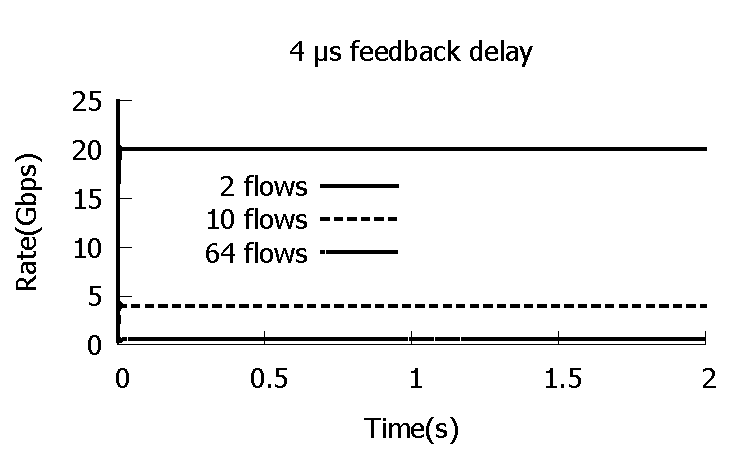
\includegraphics[width=0.49\columnwidth]{figures/stable_rate_4_pifixed.pdf}}
\subfigure[] {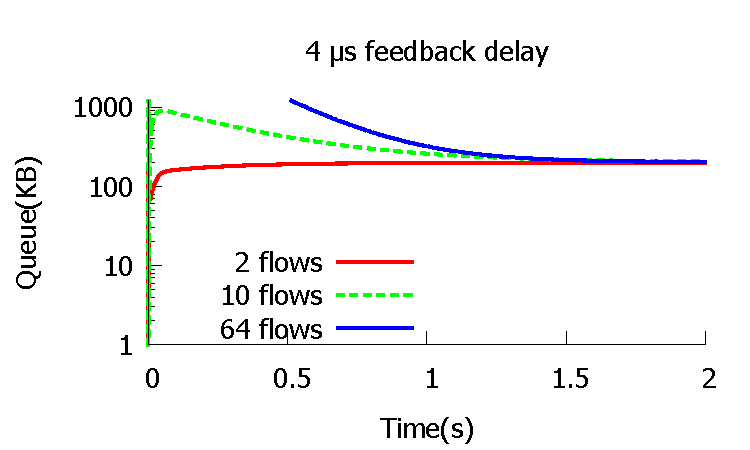
\includegraphics[width=0.49\columnwidth]{figures/stable_q_4_pifixed.pdf}}
\subfigure[] {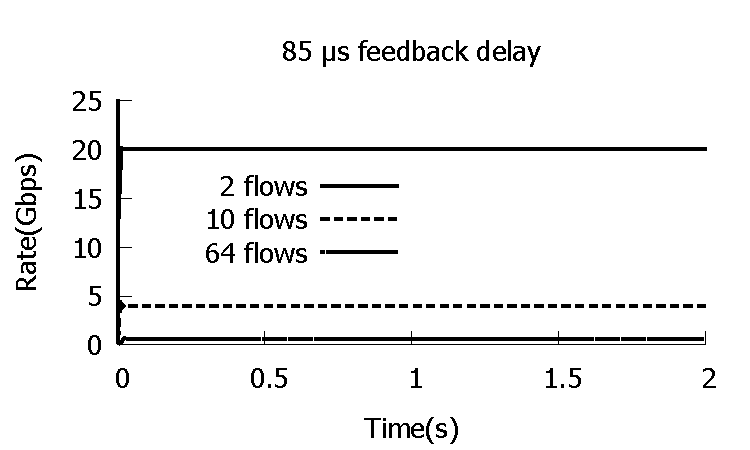
\includegraphics[width=0.49\columnwidth]{figures/stable_rate_85_pifixed.pdf}} 
\subfigure[] {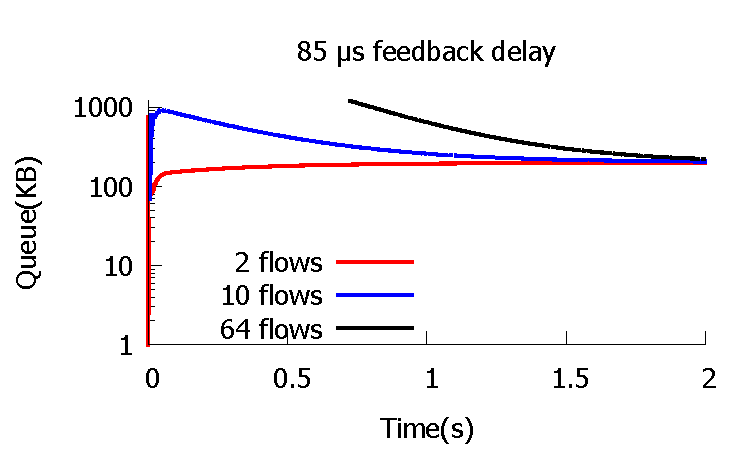
\includegraphics[width=0.49\columnwidth]{figures/stable_q_85_pifixed.pdf}}
\caption{DCQCN with PI controller}
\label{fig:dcqcn_pi}
\end{figure}

\fixme{TO DO}
In contrast, when we use a PI controller at the end hosts using delay
as the feedback signal, we see that although we can control the queue
to a specificed value, we cannot achieve fairness, as shown
in~Theorem~\ref{thm:fairness-delay}.
\begin{figure}
\center
%\includegraphics[width=0.33\textwidth]{figures/stable_timely_pi.pdf}
\caption{PI controller to stabilize TIMELY}
\label{fig:dcqcn_pi}
\end{figure}

%%% Local Variables:
%%% mode: latex
%%% TeX-master: "main"
%%% End:

\section{Related Work}
\label{sec:related}

There is a vast amount of literature on congestion control, and control
theoretic analysis of congestion control protocols of all kinds (drop-based,
delay-based, and ECN-based). For a short overview see~\cite{srikantbook}. Below,
we discuss only a few representative papers.

In~\cite{dctcp-analysis} and ~\cite{qcn-analysis}, Alizadeh et.al. analyze the
DCTCP~\cite{dctcp} and QCN~\cite{qcn} protocols that DCQCN is derived from. The
these papers served as useful guideposts during for our work.

Fluid model analysis of TCP under the RED AQM controller, and subsequent
development of the PI controller was reported
in~\cite{misra2000fluid,hollot2001designing}. Our exploration of the PI
controller for DCQCN and TIMELY is guided by results
in~\cite{hollot2001designing}.

The discussion in Section~\ref{sec:discuss} assumes that congestion control is
done on an end-to-end basis, and switches don't do much beyond marking packets.
A number of congestion control protocols where the bottleneck switch or a
central controller plays a more active role have been proposed. For example,
RCP~\cite{dukkipati2006rcp} and XCP~\cite{katabi2002congestion}~require the switches to send more detailed
feedback, while proposals like~\cite{vattikonda2012practical,wilson2011better}
use an omniscient central controller for fine grain scheduling and pFabric~\cite{pfabric}~is a timeout based congestion control that requires switches to sort packets. 

%XCP} and pFabri that


%%% Local Variables:
%%% mode: latex
%%% TeX-master: "main"
%%% End:

\vspace{-0.5em}
\section{Conclusion and future work}
We analyzed  the behavior of two recently proposed congestion control protocols
for data center networks; namely DCQCN (ECN based) and TIMELY (delay based).
Using fluid models and control theoretic analysis we derived stability regions
for DCQCN, which demonstrated a somewhat odd non-monotonic behavior of stability
with respect to the number of contending flows. We verified this behavior via
packet level simulations. We showed that DCQCN converges to a unique
fixed point exponentially. In performing similar analysis for TIMELY, we discovered that as proposed
the TIMELY protocol has infinite fixed points which could lead to unpredictable
behavior and unbounded unfairness. We provide a simple fix to TIMELY to remedy
this problem. The modified protocol is stable, and converges quickly.

However, for both protocols, the operating queue length grows with the number of
contending flows, which can introduce significant latency. Using a PI controller
on the switch to mark packets, we can guarantee bounded delay and fairness for
DCQCN.  However we demonstrate and prove a fundamental uncertainty result for
delay-based protocols: if you use delay as the only feedback signal for
congestion control, then you can either guarantee fairness or a fixed,
bounded delay,
but not both simultaneously. Based on this reason, the fact that ECN marking
process on modern shared-buffer switches effectively excludes queuing delay from
feedback loop, and that ECN is more robust to jitter in the feedback,
we conclude that ECN is a better congestion signal in data center 
environment. 

\para{Future work:} we are doing a full exploration of PI like controllers for
congestion control protocols of RDMA in the data center, including a hardware
implementation. Our analysis also suggests that DCQCN can be simplified
considerably, to remove strange artifacts like the non-monotonic stability
behavior. 

\note{We also plan to analyze problems that are not covered in the paper
due to time and space limit. These include multiple bottleneck scenario, larger 
and realistic topolgoy and workload, and the impact of PFC-induced PAUSES on 
the two protocols. To capture these complicated behaviors, we will need 
to develop more analysis tools and improve the performance of DCQCN/TIMELY NS3 
simulator~\cite{ns3rdma}.}


%%% Local Variables:
%%% mode: latex
%%% TeX-master: "main"
%%% End:


\newpage
\bibliographystyle{abbrv}
\bibliography{lossless}

\end{document}
